% =============================================================================
%  Physics of Causality
%  Pavel Sikula, Independent Researcher
%  Build:  pdflatex main && bibtex main && pdflatex main && pdflatex main
%          (or: latexmk -pdf main)
% =============================================================================
\documentclass[11pt,a4paper]{article}
% ---------------------------------------------------------------- packages
\usepackage[utf8]{inputenc}
\usepackage[T1]{fontenc}
\usepackage[safe]{tipa}
\IfFileExists{lmodern.sty}{\usepackage{lmodern}\usepackage{microtype}}{\usepackage[expansion=false]{microtype}}
\usepackage[margin=2.6cm]{geometry}
\usepackage{amsmath,amssymb,amsthm,bm}
\usepackage{booktabs,tabularx,array}
\usepackage{graphicx}
\usepackage{xcolor}
\usepackage{enumitem}
\usepackage[numbers,sort&compress]{natbib}
\usepackage[colorlinks=true,linkcolor={blue!50!black},citecolor={green!35!black},urlcolor={blue!70!black},
  bookmarksnumbered=true,bookmarksopen=true,bookmarksopenlevel=1,pdfstartview=FitH]{hyperref}
\hypersetup{pdftitle={Physics of Causality: gravity as the response of a causal order},
  pdfauthor={Pavel Sikula},
  pdfsubject={Causal sets, Benincasa-Dowker action, emergent gravity, pre-registered numerical tests},
  pdfkeywords={causal set theory; Benincasa-Dowker action; emergent gravity; non-locality; post-Newtonian gamma}}
\usepackage{url}
\setlist{itemsep=2pt,topsep=4pt}
\numberwithin{equation}{section}

% ---------------------------------------------------------------- environments
\theoremstyle{definition}
\newtheorem{axiom}{Axiom}
\newtheorem{definition}{Definition}[section]
\newtheorem{rule_}{Rule}[section]
\theoremstyle{remark}
\newtheorem*{remark}{Remark}
\newtheorem*{status}{Status}

% a box for the verdict of a laboratory test
\newcommand{\verdict}[1]{\textsc{#1}}
% status label of a statement in the ontology part
\newcommand{\stat}[1]{\unskip\nobreak\hfill\mbox{\footnotesize\textsf{[#1]}}}
% editorial notes (to be removed before publication)
\newcommand{\todo}[1]{\textcolor{red}{[TODO: #1]}}

% ---------------------------------------------------------------- notation
\newcommand{\lk}{\ell_k}
\newcommand{\Pib}{\Pi}
\newcommand{\dd}{\mathrm{d}}
\newcommand{\BD}{\mathrm{BD}}
\newcommand{\Khat}{\hat K}
\newcommand{\Ex}{\mathbb{E}}
\renewcommand{\vec}[1]{\bm{#1}}
% coefficients of the static quadratic form of the action of the order (Einstein--Hilbert: 6, 8, 2)
\newcommand{\cA}{\mathcal{A}}
\newcommand{\cB}{\mathcal{B}}
\newcommand{\cC}{\mathcal{C}}


\title{Physics of Causality\\[4pt]
\large Gravity as the response of a causal order: from a Lorentz-invariant substrate\\
to the Einstein--Hilbert stiffness of the Benincasa--Dowker action}
\author{Pavel \v{S}ikula\\ \small Independent Researcher, Brno, Czech Republic\\ \small ORCID: \todo{ORCID}}
\date{October 2026}

\begin{document}
\maketitle
\begin{abstract}
\noindent
Causal Physics takes the causal order of events, not spacetime geometry, as the primitive of physics.
We formulate it so that every step can be confronted with a pre-registered numerical test, and we
report the outcome of these tests, positive and negative.

\smallskip\noindent
\textbf{Substrate.} The tests decide the nature of the substrate. A discrete substrate with a
finite number of neighbours per event and a rest frame is not supported; the substrate is a
Lorentz-invariant causal set, a Poisson sprinkling in which geometry is read from order and number.
Matter is a flow of events that carries its own four-velocity, and the action of a flow is its proper
time as counted by the order.

\smallskip\noindent
\textbf{Gravity as the response of the order.} Near matter the order changes: clocks slow down, causal
cones narrow and events become denser. A fixed order gives the scalar (Nordstr\"om) class
$\gamma=-1$, cones that only narrow give $\gamma=1/d_s$, and an order that conserves its causal
throughput gives $\gamma=2/(d_s-1)$, which is $\gamma=1$ exactly in three spatial dimensions. In
3+1 dimensions this throughput principle is the linearised coupling of general relativity to the full
energy--momentum tensor. A substrate rule in which every flow narrows the cone in its own rest
frame and capacity deficits add reproduces this coupling on 3+1 sprinklings: two counter-streaming
beams gravitate with the predicted active mass ($2.40\pm0.05$ against $2.36$, alternatives $1.56$
and below), the cones become anisotropic and a single beam drags them.

\smallskip\noindent
\textbf{The rule from the action of the order.} With proper time counted by the order, the substrate
rule is the linear response of an order whose action has the Einstein--Hilbert stiffness. We compute
the expectation value of the smeared Benincasa--Dowker action of a causal set to second order in a
static perturbation, in 3+1, by deterministic quadrature with nothing from general relativity put in.
The Einstein--Hilbert stiffness emerges in the conformal sector, $6.0003$ against $6$, and in the mixed
sector, where the perturbation changes the causal order itself, $7.983$ against $8$, and in the optical
sector, where rays bend, $2.002$ against $2$. With all three coefficients $\gamma=1$ follows from the action of
the order ($0.997$ to $1.000$). The discreteness corrects the stiffness non-analytically, $1-\hat K\simeq(k\ell_k)^2[4.0\ln(1/k\ell_k)+0.9]$, and adds a
non-local term that grows with the age $T$ of the static field, $-0.10\,(k\ell_k)^3T/\ell_k$, which
we predicted analytically before computing it.

\smallskip\noindent
\textbf{Predictions.} Beyond the leading order the sectors differ, and each weakens with the age $T$ of a
static field: linearly in the conformal and mixed sectors, faster than linearly in the optical sector within
the computed range. The age terms are not suppressed like the local corrections: if the age of a static field
is cosmological, a non-locality scale at the level of existing bounds, $\ell_k\sim10^{-19}$\,m, places the
breakdown of the static response at tens of micrometres or above, within reach of torsion balances. The
asymptotic form of the optical age term, which fixes the far-field law of a point mass, is the next
computation. Beyond the linear order the theory is completed by general relativity, to be
derived thermodynamically; strong-field predictions of a scalar field equation are therefore not
predictions of the theory. Every result quoted here is reproducible with the open Causality
Lab~\cite{CausalityLab}, including the negative ones.
\end{abstract}

\tableofcontents
\clearpage

% =============================================================================
\section{Introduction}\label{sec:intro}
% =============================================================================

\subsection{Causality before geometry}

General relativity treats spacetime geometry as dynamical but primary; quantum field theory treats it
as fixed and equally primary. In both, matter and fields evolve on a manifold that exists before
anything happens on it. Causal Physics adopts the opposite stance: the primitive of physics is a
set of events and the relation of influence between them,
\begin{equation}
  u \prec v \quad\Longleftrightarrow\quad u \text{ can influence } v ,
\end{equation}
and geometry is a large-scale description of regularities in that relation.

This stance is not new. It is the founding hypothesis of causal set theory, compressed by Sorkin
into the slogan ``order $+$ number $=$ geometry''~\cite{Bombelli1987,Surya2019}: a causal order
determines a Lorentzian metric up to a conformal factor, and the number of events in a region
fixes that factor. What Causal Physics adds is a physical reading of the order. Events are updates
of a substrate; persistent flows of events are matter; and gravity is the way the order itself
responds to those flows, slowing clocks, narrowing causal cones and adding events near matter. The
question this paper asks is how much of gravitation follows from that picture once it is made
precise enough to be computed.

\subsection{Method: a laboratory that tests and does not rescue}\label{sec:method}

All quantitative statements in this paper come from the Causality Lab~\cite{CausalityLab}, an open
collection of numerical tests written for this programme. The rules of the laboratory matter as
much as its results, because a theory developed together with its own tests can easily test only
what it already put in.

Every test states its question, prediction, null model and numerical criterion before the full run,
declares the level of conclusion it can support, and ends with one of four verdicts:
\verdict{passed}, \verdict{failed}, \verdict{undecided} or \verdict{instrument failed}. Negative
results are kept, and a failed test is never rescued by changing its criteria. The rules are stated
in full as the methodological principles M1--M7 (Sec.~\ref{sec:method-ax}).

Throughout the paper, results are labelled with the identifiers of the tests (e.g.\ F7.4a) so that
each can be rerun. Appendix~\ref{app:lab} lists the tests used.

\subsection{Main results}

\begin{enumerate}
\item \textbf{The substrate} is a Lorentz-invariant causal set; a finite-degree substrate with a rest
  frame is excluded by the tests together with a known theorem (Sec.~\ref{sec:substrate}).
\item \textbf{Geometry is read blindly from the order.} An instrument that receives only events
  and their relation recovers the clock potential $\phi$ and the spatial potential $\psi$ of a weak
  field, and with them the post-Newtonian parameter $\gamma$, in 2+1 and 3+1 dimensions
  (Sec.~\ref{sec:reading}).
\item \textbf{Matter carries momentum.} A flow that keeps its timelike direction as a state stays
  localised and moves with its source, and its energy--momentum tensor is measured correctly
  (Sec.~\ref{sec:flows}).
\item \textbf{The response of the order fixes $\gamma$.} A fixed order gives $\gamma=-1$, narrowing
  cones alone give $\gamma=1/d_s$, and conservation of causal throughput gives
  $\gamma=2/(d_s-1)$; on 3+1 sprinklings the last reads $\gamma=1.000\pm0.045$ (raw value; the
  formal verdict is undecided because the comparison metric was read with a larger error,
  Sec.~\ref{sec:response}).
\item \textbf{The coupling is tensorial.} In 3+1 the throughput principle is the linearised coupling
  of general relativity to $T_{ab}$; a substrate rule realising it makes pressure and motion
  gravitate and drags the cones (Part~\ref{part:geometric}).
\item \textbf{The rule follows from the action of the order.} The expected Benincasa--Dowker action
  of a causal set carries the Einstein--Hilbert stiffness in the static conformal sector,
  $6.0003$ against $6$, in the mixed sector, $7.983$ against $8$, and in the optical sector, $2.002$
  against $2$; $\gamma=1$ follows ($0.997$ to $1.000$). The discreteness adds a non-analytic correction and
  non-local age terms (Part~\ref{part:geometric}).
\item \textbf{The road to predictions} is the static quadratic form of the order, now known in all three
  sectors; the asymptotic age term of the optical sector is the next computation
  (Part~\ref{part:predictions}).
\item \textbf{Where to look.} The age term is not suppressed like the local corrections. For a cosmological
  age and $\ell_k$ at the level of existing bounds it places the breakdown of the static response at tens of
  micrometres, the range of current torsion balances (Sec.~\ref{sec:window}).
\end{enumerate}

\subsection{Relation to existing frameworks}

\paragraph{Causal set theory.} The substrate, the reading of geometry from order and number and the
Benincasa--Dowker operator and action are taken from causal set
theory~\cite{Bombelli1987,Surya2019,BenincasaDowker2010,Sorkin2007,DowkerGlaser2013}. The
contribution of this work lies elsewhere: in the physical reading of matter as flows that carry
momentum, in the principle by which the order responds to them, in the explicit second-order
computation of the expected action with its non-local age term, and in the systematic numerical
testing of each step.

\paragraph{General relativity.} The theory does not compete with general relativity in the regime
where general relativity is tested. In the linear regime it reproduces it, and beyond the linear
order it adopts it, with the intention of deriving it thermodynamically along the lines of
Jacobson~\cite{Jacobson1995}. Its own content lies in the discreteness and non-locality of the
substrate.

\paragraph{Uniqueness theorems.} A massless spin-2 field coupled consistently to the total conserved
energy--momentum is general relativity~\cite{Deser1970,FeynmanGravitation}, and in four dimensions
the Einstein tensor is the unique divergence-free tensor built from the metric and its first two
derivatives~\cite{Lovelock1971}. The results of Part~\ref{part:geometric} are consistent with these
theorems and use them: once the order is shown to couple to $T_{ab}$ with the Einstein--Hilbert
stiffness, the non-linear completion is fixed.

\paragraph{Modified gravity.} The theory makes no claim of a modified low-acceleration regime
(Sec.~\ref{sec:astro-cosmo}).

\subsection{Structure of the paper}

Part~\ref{part:ontology} describes, without equations, how Causal Physics sees the world: events,
order and time, observation, transport, merging, matter, gravity, horizons and superposition, each
statement labelled by how firmly it stands. Part~\ref{part:foundations} sets up the substrate, the reading of geometry from it, matter as flows
and the response of the order. Part~\ref{part:units} states the parameters and the conditional
bridge to SI units. Part~\ref{part:axioms} collects the axioms in their revised form, with the status
of each. Part~\ref{part:geometric} derives and tests the gravitational coupling, from the throughput
principle to the Einstein--Hilbert stiffness of the discrete action. Part~\ref{part:astro} states what
remains of the strong-field and astrophysical claims. Part~\ref{part:predictions} sets out the
predictions the theory can make and how they can fail. Part~\ref{part:discussion} discusses the
limitations. Appendix~\ref{app:lab} describes the laboratory and the tests;
Appendix~\ref{app:changes} relates this formulation to the first published version of the
programme.


\part{The Causal Picture of the World}\label{part:ontology}
% =============================================================================
%  Part II -- The causal picture of the world (ontology)
% =============================================================================

This part describes the world as Causal Physics sees it, in words rather than equations. It follows
one line of thought: from what exists, through time, space and motion, to matter, gravity and the
limits of what can be known. The mathematics of the following parts is a precise form of this
picture. Each statement carries a label that says how firmly it stands:
\textsf{[tested]} -- supported by a test of the laboratory (identifier given);
\textsf{[derived]} -- follows from a derivation in this paper or from established results it uses;
\textsf{[observed]} -- seen in a test, but not the outcome the test judged;
\textsf{[interpretation]} -- a reading consistent with the results, from which nothing is computed;
\textsf{[open]} -- part of the programme, not yet formulated or tested.

% =============================================================================
\section{What exists: events and influence}\label{sec:onto-events}
% =============================================================================

The world is not made of things that exist in space and persist in time. It is made of
\emph{events}: elementary happenings, each of which is an act of realisation. An event has no size,
no position, no mass and no charge. What it has is relations: some events can influence it, and it
can influence others. Everything we call a property, the position of a stone, the mass of a planet,
the tick of a clock, is a pattern in these relations, visible only when many events are taken
together. \stat{interpretation}

The single primitive relation is \emph{influence}: one event can affect another. Influence has a
direction, and it never closes into a loop: nothing influences its own past. With these two facts
the set of all events becomes an \emph{order}, and the order is the deepest structure of the world.
Everything else in this part is a way of reading it. \stat{derived}

A table, in this picture, is not an object that happens to be at a place. It is a pattern of events
that keeps reproducing itself, update after update. Its solidity is the stability of the pattern,
and its place is the way the pattern is woven into the surrounding web of influence.
\stat{interpretation}

% =============================================================================
\section{Time: the order seen from inside}\label{sec:onto-time}
% =============================================================================

``Earlier'' means ``could have influenced''; ``later'' means ``could have been influenced by''. Time
is nothing more than this. There is no universal now: two events that cannot influence each other
have no fact about which came first, and no observer can find one. \stat{derived}

Each observer has a local time, the number of events along their own history. A clock is a pattern
that repeats, and its ticks are counted events. The clocks of two observers agree only where their
histories are related, and they need not agree on how much time has passed between two meetings.
\stat{derived}

The passage of time is the growth of the order. New events appear in the future of existing ones and
never in their past. The past is fixed because it has already been realised; the future is open
because it has not. \stat{interpretation}

% =============================================================================
\section{Space and dimension}\label{sec:onto-space}
% =============================================================================

Space is what lies between events that cannot influence each other. A ``moment'' of the world, as
an observer experiences it, is a large set of mutually unrelated events, and the distances within it
are read from how far one has to go into the past or the future to find events related to both. Space
is therefore not a container that exists first; it is the side-by-side structure of the order.
\stat{derived}

The order fixes the shape of spacetime up to a local scale, and counting events fixes the scale.
Nothing else is needed: distances, volumes, the rate of clocks and the dimension itself are read
from order and number. The dimension, for example, is visible in what fraction of pairs of events
in a region are related. \stat{tested: K.1, K.16b, K.16c}

Why space has three dimensions is not derived here. But it is notable that the way the order responds
to matter (Sec.~\ref{sec:onto-gravity}) agrees with the gravity we observe in exactly three spatial
dimensions and in no other. \stat{derived}\quad Whether this is the reason for three dimensions is
an open question. \stat{open}

% =============================================================================
\section{Motion and relativity}\label{sec:onto-motion}
% =============================================================================

The substrate looks the same to every observer moving uniformly. There is no state of rest in it, no
ether against which motion could be measured, and no experiment can find one. This is the principle of
relativity, and here it is a property of the substrate, not an additional postulate.
\stat{derived}

The speed of influence is the same for all observers for the same reason: the boundary between
events that can and cannot influence each other is part of the order, and the order is the same for
everyone. The speed of light is the conversion between counting events along time and counting them
across space. \stat{derived}

A moving clock runs slow because it takes a shorter path through the order. Between two meetings,
the observer who stays at rest passes through the longest chain of events, and an observer who
travels away and comes back passes through fewer. The travelling twin is younger because fewer
events happened to her, not because anything acted on her clock. \stat{derived}

% =============================================================================
\section{Observing is receiving causes}\label{sec:onto-observe}
% =============================================================================

To observe something is to be on the receiving end of its influence. Seeing a tree means that
events in the tree have influenced, through a long chain of intermediate events, the events of our
eye. There is no observation without causal contact, and every observation is itself an event that
joins the order.

This explains why the world looks different near and far. A tree next to us is rich in detail; the
same tree on the horizon is a silhouette. The tree has not changed. What has changed is the density
and fidelity of the influence that connects it to us. Two different effects are at work.
\begin{itemize}
\item \emph{Geometric dilution.} The same influence spreads over a larger sphere as it travels, so
  less of it reaches us, in proportion to $1/r^2$. This is the root of the inverse-square law.
  \stat{tested: F1.1}
\item \emph{Loss through intermediaries.} Where influence passes through many intermediate events
  (air, dust, memory, a historical record), each of them reshuffles it, and detail is lost. This is
  the entropic side of distance. \stat{interpretation}
\end{itemize}
Influence that travels through empty space along the light cone does not pass through intermediaries
in this sense: events on the light cone are causally close however distant they are in space. The
images of very distant point sources are therefore not blurred by the discreteness of the substrate,
and the sharp images of distant quasars agree with that. \stat{derived}

% =============================================================================
\section{Scale and causal resolution}\label{sec:onto-scale}
% =============================================================================

What we call scale is the resolution with which the order can be read. Different physical regimes
are different limits of that resolution, not different sizes.

\paragraph{The discreteness scale.} At the scale of individual events the order is well defined, but
there are too few events in any region to fix a shape. Trajectories, fields and distances lose their
meaning here, and only the relations remain. \stat{derived}

\paragraph{The plateau.} When regions contain many events and the order is close to a uniform
sprinkling, geometry becomes an excellent compression of it. This is the regime of ordinary matter
and of everyday experience, in which three-dimensional space and Lorentzian spacetime are reliable
descriptions. Dynamics of orders of this kind has a phase whose typical members look like spacetime,
separated by a transition from phases that do not.
\stat{known in 2D~\cite{Surya2012}; in part F6.4a}\quad
General relativity and quantum field theory are effective descriptions on the plateau.
\stat{interpretation}

\paragraph{Between the two.} At an intermediate scale $\ell_k$ the order is smooth enough for
geometry but still remembers that it is discrete. Its response reaches along the light cone to
distant events, and the response to a static field depends on how long that field has existed.
\stat{derived, Sec.~\ref{sec:bdaction}}

% =============================================================================
\section{Transport: nothing from nothing}\label{sec:onto-transport}
% =============================================================================

The substrate is not a passive stage. It carries influence from events to the events they affect,
and this influence is conserved: what flows into an event flows out of it, apart from what the event
stores. Nothing appears from nothing and nothing disappears into nothing. This continuity is the
most basic law of the substrate, and the conservation laws of physics are its large-scale
expressions. A steady source surrounded by any closed surface sends exactly its own output through
it, which is Gauss's law. \stat{tested: F1.1}

The capacity of an event to pass influence on is finite. When more influence arrives than an event
can carry, it is held back: the substrate buffers it, and an observer sees this as delay. Delay is
not a defect of transmission but the visible expression of a finite causal bandwidth.
\stat{interpretation}

% =============================================================================
\section{Branching, merging and the meaning of energy}\label{sec:onto-merging}
% =============================================================================

Influence branches and merges. \emph{Branching} distributes the influence of one event among many
later events. \emph{Merging} compresses influence that arrived along distinct paths into a single
continuation. At the level of the substrate the two are symmetric: every event is a meeting point of
its past and a source of its future. \stat{interpretation}

\paragraph{Energy.} The amount of influence carried is \emph{energy}; the direction in which it is
carried is \emph{momentum}. Together they are one quantity seen from different frames: energy is the
part along time, momentum the part across space. Both are conserved because influence is.
\stat{tested: K.15}

\paragraph{Mass.} When two streams of influence moving in different directions merge, their directed
motion is not lost. It becomes internal: the merged stream moves more slowly as a whole and carries
more rest energy, in exactly the proportion that conserves energy and momentum together. Merging is
how motion becomes mass and heat; two counter-streaming populations that merge cool down. Mass is
energy that no longer points anywhere. This is the content of $E=mc^2$ in this picture.
\stat{tested: K.15, F4.1}

% =============================================================================
\section{Light and matter}\label{sec:onto-matter}
% =============================================================================

\paragraph{Light.} Influence that travels on the boundary of the order, along the light cone, has no
clock: no events happen along its way, it cannot be at rest, and it has no rest frame. Light is
influence in pure transit. \stat{derived}

\paragraph{Matter.} Matter is influence that persists. A flow that only spread out would be radiation:
it would fill its light cone and dissolve. A flow that stays together, carried from event to event
along a narrow bundle of histories, is matter, and along its history events happen: matter has
clocks.

What keeps a flow together on a substrate that has no preferred directions is \emph{memory}. A flow
that carries its own direction of motion as a state passed from event to event stays on the world line
of its source and moves with the source when the source moves. This memory of direction is
\emph{inertia}: a body continues in its motion because its flow remembers where it was going.
Momentum is not added to matter from outside; it is what makes localised matter possible at all.
\stat{tested: F3.6}

\paragraph{Structure.} Where repeated activity keeps routing influence through the same region, the
substrate approaches its capacity and influence can no longer spread freely: it is confined to a
restricted set of paths. Structure is the self-maintaining outcome of this confinement, a dynamical
equilibrium between the continuity of influence and the finiteness of capacity, maintained as long as
the activity that creates it continues. \stat{interpretation}\quad How such confinement closes into
a self-bound object, a particle that holds itself together without an external source, is the central
open problem of the matter sector. \stat{open}

% =============================================================================
\section{Gravity: the order responds to matter}\label{sec:onto-gravity}
% =============================================================================

\paragraph{Load.} Matter is a flow that passes through the substrate continuously, and the substrate
carries it as load. A loaded substrate does three things at once: its clocks run slower, because more
of its activity goes into carrying the flow; its causal cones narrow, because influence travels more
slowly through it; and it becomes denser, because it adds events.
\stat{effects derived; reasons: interpretation}

\paragraph{Throughput.} The last two effects are tied together by one principle, familiar from traffic
and from every conserved current passing through a constriction: \emph{the throughput is conserved}.
Where cars slow down they bunch up, so that the number passing a point per minute stays the same.
Where the substrate slows influence down, it adds events, so that the number of events a light front
passes per unit time and area stays the same. The speed of light is the maximal rate at which
influence travels without congestion; near matter the effective speed falls below it.
\stat{derived; tested: F7.1c}

\paragraph{The field.} The response of the order is not confined to where the matter is. It spreads,
at the speed of influence, into the surrounding substrate, weakening with distance as influence does.
The gravitational field is this spreading response of the order: not a substance added to spacetime,
but the order itself, reshaped. \stat{tested: F1.3}

\paragraph{Falling.} A body falls because its history bends towards slower clocks: of all histories
between two events, matter follows the one along which the most events happen, and near a mass that
history leans towards the mass. Light bends because the cones it travels along narrow towards
matter. The amount by which light bends, twice what a naive Newtonian picture gives, is exactly what
the conservation of throughput gives in three spatial dimensions. \stat{derived; fall from the order: 2+1 passed (F5.1d), 3+1 failed (F5.1e)}

\paragraph{Equivalence.} All bodies fall in the same way, whatever they are made of, because falling is
not a reaction to a force but the following of the order's own longest histories. What a body is made
of does not enter into which history is longest. Being pushed and being attracted probe the same
property of the substrate from two sides. \stat{derived}

\paragraph{Everything that moves gravitates.} The substrate responds to a flow in the flow's own rest
frame, and the responses of different flows add. Because of this, not only mass but also pressure
and motion gravitate, and a moving flow drags the causal cones along with it.
\stat{tested: F7.4a}\quad The order responds in this way because its own dynamics, the action that
counts its intervals, has exactly the stiffness of Einstein's gravity.
\stat{derived and computed, Sec.~\ref{sec:bdaction}}

\paragraph{Non-linearity.} Weak fields add. Strong ones do not: when two sources sit close together,
each lies in the well of the other and acts more weakly, so the common well is shallower than the sum
of the two. Gravity is non-linear because the order responds to its own response.
\stat{tested: F1.4}

% =============================================================================
\section{Horizons and the limits of reconstructability}\label{sec:onto-horizons}
% =============================================================================

Where the substrate is loaded very strongly, geometry stops being a good description of the order.
The events are still there and influence still flows, but the order no longer behaves like a smooth
spacetime: reading it with clocks, cones and densities gives answers that do not fit together into
one metric. \stat{observed: F7.1b}

A \emph{causal horizon} is the limit of reconstructability: the boundary beyond which an external
observer can no longer keep an order-preserving description of what happens inside using a global
time, a smooth geometry or isotropic propagation. Beyond it, causal updates continue without
interruption and causal continuity is intact. What is lost is the ability to describe the inside in
the language of the outside. Horizons mark the reach of geometric language; they are not a boundary
of causal evolution itself. \stat{interpretation}

Merging plays a central role here. When many causal channels converge under extreme load, the causal
distance between events collapses from the substrate's own point of view. To an observer who relies on
geometric reconstruction, this collapse appears as temporal ambiguity, loss of detail and horizon
behaviour. \stat{interpretation}

% =============================================================================
\section{Entropy and the arrow of time}\label{sec:onto-entropy}
% =============================================================================

The order has a direction because it grows: events are added to its future, never to its past. This
is the deepest arrow of time. \stat{interpretation}

Merging gives the arrow a second, familiar face. Branching can be followed backwards: every branch
remembers where it came from. Merging cannot be undone uniquely: once distinct paths have joined
into one continuation, many different pasts are compatible with the same present. What is lost is
the record of which past it was, and the measure of that loss is \emph{entropy}. Irreversibility is
the asymmetry between how easy it is to merge and how hard it is to unmerge. \stat{interpretation}

A horizon carries an entropy proportional to its area, and the order counts it directly: the number
of pairs of events that straddle the horizon in a minimal way is proportional to its proper area.
\stat{tested: K.14}\quad This is the bridge to the thermodynamic view of gravity, in which Einstein's
equations describe the equilibrium of the order the way the gas laws describe the equilibrium of
molecules. \stat{open, Sec.~\ref{sec:jacobson}}

% =============================================================================
\section{The vacuum is not empty}\label{sec:onto-vacuum}
% =============================================================================

Empty space is not nothing. It is the substrate with no flow through it: events at their fundamental
density, related to each other in the way that makes a flat spacetime. Every region of vacuum contains
a definite number of events, and that number fluctuates as counts do, by about its square root.
\stat{derived}

Such fluctuations of number act on the large-scale geometry like a small cosmological constant whose
size is set by the volume of the observable universe; for the present universe it is of the order of
the observed value~\cite{Ahmed2004}. In Causal Physics this would make dark energy the residue of the
discreteness of the substrate. \stat{open}

The growth of the order on the largest scale is the natural candidate for the expansion of the
universe. \stat{open}

% =============================================================================
\section{Superposition and measurement}\label{sec:onto-superposition}
% =============================================================================

An event can have several admissible continuations, and as long as nothing distinguishes them they
coexist. In Causal Physics there is no separate collapse process; there is stabilisation under
interaction.
\begin{itemize}
\item \emph{Superposition} is the coexistence of admissible causal continuations.
\item \emph{Measurement} is a causal interaction that biases the routing of influence towards one of
  them.
\item \emph{Collapse} is the stabilisation of a single continuation. It is irreversible because
  undoing it would require a coordinated redistribution of influence across an extended region of the
  substrate, and the growing impedance of that region suppresses it. It is a merging that cannot be
  undone.
\end{itemize}
At the discreteness scale, where patterns do not persist long enough to be compressed into
trajectories, every observation perturbs what it probes. Quantum behaviour is then the behaviour of a
substrate that is too unstable for geometric compression, rather than a paradox of measurement.
\stat{interpretation}\quad A quantum dynamics of the order that would make this picture quantitative
is not part of the present work. \stat{open}

% =============================================================================
\section{The frontier}\label{sec:onto-missing}
% =============================================================================

Persistent currents of influence that circulate rather than stream are natural candidates for
\emph{charge} and \emph{spin}: asymmetries in how influence is routed around a structure, invisible from
far away except through their effect on routing. The freedom to relabel routes without changing any
observable flow would then be the origin of \emph{gauge freedom}. These ideas belong to the programme;
none of them is formulated or tested here. \stat{open}

% =============================================================================
\section{The picture in one paragraph}\label{sec:onto-summary}
% =============================================================================

The world is a growing order of events. Its direction is time, its side-by-side structure is space,
and its sameness for every observer is relativity. Influence flows through it and is conserved; its
amount is energy and its direction is momentum. Influence that persists and remembers its direction is
matter, and that memory is inertia; influence in pure transit is light. Matter loads the order, and
the order responds by slowing its clocks, narrowing its cones and adding events so that its throughput
is kept: that response, spreading outwards, is gravity. Where the load is extreme, geometry can no
longer describe the order, and a horizon marks the limit of what the outside can reconstruct. What
cannot be unmerged is entropy, and what has not yet been stabilised is superposition. From events to
gravity each step is tested or derived; self-bound matter, charge, spin and the quantum are the
frontier.


\part{Causal Physics on a Lorentz-Invariant Substrate}\label{part:foundations}
% =============================================================================
\section{The substrate}\label{sec:substrate}
% =============================================================================

\subsection{Events, order and number}

The primitive objects are \emph{events}. An event carries no position, duration, mass or charge;
everything is relational. Events are connected by a relation of influence $\prec$ that is
\begin{itemize}
\item \emph{transitive}: $u\prec v$ and $v\prec w$ imply $u\prec w$;
\item \emph{acyclic}: $u\prec v$ and $v\prec u$ never hold together (no closed causal loops);
\item \emph{locally finite}: between any two events there are finitely many others.
\end{itemize}
A set with such a relation is a causal set~\cite{Bombelli1987,Surya2019}. Two derived notions carry
most of the physics:
\begin{itemize}
\item the \emph{interval} $I(u,v)=\{w: u\prec w\prec v\}$ and its number of elements $n(u,v)$;
\item the \emph{chains} $u\prec w_1\prec\dots\prec v$; the length of the longest chain between $u$ and
  $v$ is a discrete proper time.
\end{itemize}

When the causal set is faithfully embedded in a Lorentzian manifold $(M,g)$, the relation $\prec$ is
the causal order of $g$ and the number of elements in a region is, on average, $\rho$ times its
spacetime volume. The order fixes the metric up to a local scale; the number fixes the scale.
The standard realisation is a \emph{sprinkling}: a Poisson process of density $\rho$ per unit proper
volume, with the relation inherited from the light cones of $g$. A sprinkling is statistically
invariant under Lorentz transformations: there is no preferred frame in which it looks different
from any other.

\subsection{Why the substrate must be Lorentz invariant}\label{sec:why-lorentz}

A natural alternative is a graph in which each event has at most $K_0$ relations, locality is
distance in the graph and time is the count of updates. Such a substrate has a rest frame. A Lorentz-invariant discrete structure cannot have it: in a sprinkling every event is related
to infinitely many others along its light cone (finitely many only because a simulated region has a
wall), and no Lorentz-invariant rule can select a finite set of neighbours
locally~\cite{BombelliHensonSorkin2009}. Finite degree and Lorentz invariance of the substrate
exclude each other.

There are two options. (A) A Lorentz-invariant substrate: relativity comes for free and
non-locality is unavoidable. (B) A substrate with a rest frame: Lorentz invariance must emerge for
observers with extreme precision, and small violations at the discreteness scale tend to be
amplified by quantum corrections. The tests of the laboratory support (A)
(Appendix~\ref{app:lab}):
\begin{itemize}
\item the degree of an event grows with the number of events in the region; a bound $K_0$ does not
  hold (F0.3);
\item capacity limits the \emph{flow} through an event, not the number of its relations (F1.8;
  supported, but not robust to the seed);
\item local growth rules of the finite-degree type produced no manifold-like order (0 of 7 rules,
  F6.1) and no three-dimensional space (F6.2).
\end{itemize}
The substrate of Causal Physics is therefore a causal set. Capacity survives as a bound on the flow that an event
can carry (Part~\ref{part:axioms}).

\subsection{Non-locality}

Because every event is related to events arbitrarily far away along its light cone, local
differential operators have no direct discrete analogue. The causal set d'Alembertian of Benincasa
and Dowker~\cite{BenincasaDowker2010}, in its smeared form due to Sorkin~\cite{Sorkin2007}, sums
over the whole causal past of an event with weights that depend on the number of elements in each
interval. The smearing introduces a non-locality scale
\begin{equation}
  \ell_k=(\epsilon\rho)^{-1/D},
\end{equation}
where $D$ is the spacetime dimension and $0<\epsilon\le1$ the smearing parameter. For $\epsilon=1$,
$\ell_k$ is the discreteness scale itself; for small $\epsilon$ it is larger. The operator is defined in
Sec.~\ref{sec:bd}; its non-locality is a physical property of the substrate, and one of the results of
this paper (Part~\ref{part:geometric}) is a non-local term in the action that it implies.

% =============================================================================
\section{Reading geometry from the order}\label{sec:reading}
% =============================================================================

A theory in which geometry is emergent must say how geometry is read. For a weak static field in
isotropic coordinates,
\begin{equation}\label{eq:weakmetric}
  \dd s^2=-e^{2\phi}\,\dd t^2+e^{-2\psi}\,\dd\vec x^2,\qquad \gamma=\psi/\phi,
\end{equation}
($\phi$ the clock potential, $\psi$ the spatial potential, $\gamma$ the post-Newtonian parameter),
three quantities of the order determine both potentials:

\begin{center}
\begin{tabular}{lll}
\toprule
quantity of the order & what it measures & weak-field value\\
\midrule
clocks: elements of a small interval at rest & proper time & $\phi$\\
the boundary of the relation & speed of the causal cone $c$ & $\phi+\psi$\\
density of elements per coordinate volume & $\sqrt{-g}$ & $\phi-d_s\psi$\\
\bottomrule
\end{tabular}
\end{center}
($d_s$ is the number of spatial dimensions.) Any two of the three determine $\gamma$; the third is a
consistency check that the order is metric at all.

\paragraph{The blind instrument.} The laboratory built an instrument that receives only the events,
the relation and the fundamental density, not the metric, and reads $\gamma$ along two independent
paths: (A) cones and density, (B) clocks and cones. It was calibrated on orders sprinkled into
metrics with known $\gamma$ (K.16b in 2+1, K.16c in 3+1). In 2+1, for a field
$\phi=-0.1\,e^{-r^2/128}$, it returns $-1.000\pm0.001$ for $\gamma=-1$, $-0.04\pm0.02$ for $\gamma=0$
and $+0.92\pm0.03$ for $\gamma=+1$. In 3+1 it returns $-1.001\pm0.001$, $0.33\pm0.04$ and
$0.99\pm0.05$ for $\gamma=-1,\ 1/3,\ +1$. For fields weaker than $|\phi|\sim0.03$ the instrument is
unreliable; all tests that use it work with $|\phi|\sim0.1$. The instrument uses coordinates and
the known density as a declared readout; a coordinate-free reading (radar echoes) is a planned
improvement. Figure~\ref{fig:blind} shows the calibration and the potentials read by radius.

\begin{figure}[t]
  \centering
  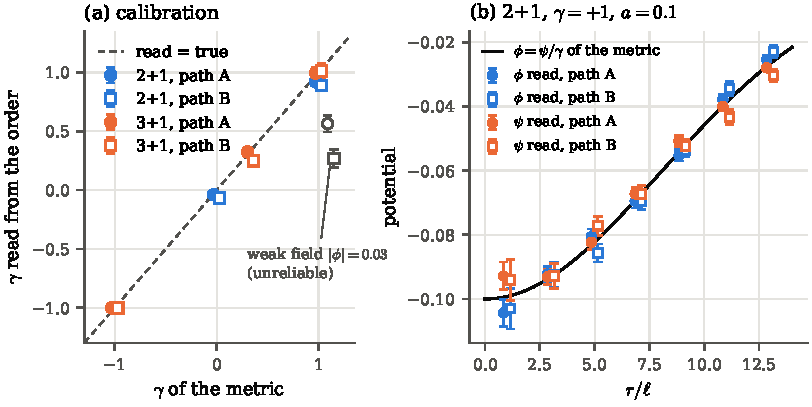
\includegraphics[width=\textwidth]{figures/fig_blind.pdf}
  \caption{The blind instrument (K.16b, 2+1; K.16c, 3+1). (a) $\gamma$ read from orders sprinkled into metrics of known
$\gamma$, along path A (cones and density, filled) and path B (clocks and cones, open); grey: the weak field
$|\phi|=0.03$, where the instrument is unreliable. (b) The potentials read by radius for $\gamma=+1$ in 2+1
($a=0.1$, $\psi=\phi$) against the profile of the metric. Bars: $\pm1$ standard error over 32 (2+1) and 16 (3+1)
sprinklings.}\label{fig:blind}
\end{figure}

\paragraph{Other instruments.} The clock rate $\Pi$ can be read back from the density of chains
(K.3); the causal front of a source measures the Shapiro delay to within $2\%$ of the general
relativistic value (K.2); and the number of ``horizon molecules''~\cite{DouSorkin2003,Barton2019}
measures the area of a horizon in flat space in 1+1, 2+1 and 3+1 dimensions and its \emph{proper} area in
a conformally flat geometry, with the exponent of the proper-area law $1.96\pm0.06$ against $2$ in 3+1 (K.14). The last instrument is the entropy meter of the
thermodynamic route of Sec.~\ref{sec:jacobson}.

% =============================================================================
\section{Matter as flows}\label{sec:flows}
% =============================================================================

\subsection{Flow and its conservation}

Matter in Causal Physics is a persistent pattern of events. Its simplest model is a \emph{flow}: a
non-negative quantity $F$ transported from events to their successors along the relations of the
order and conserved at every event (Axiom~\ref{ax:continuity}). A steady source then obeys Gauss's
law: the flow through any closed surface around it equals the source, $J/S=1.003$--$1.004$ in 2+1 and
3+1 with up to $2.6\times10^5$ events, against $0.77$--$0.88$ for a model without conservation (F1.1).

\subsection{A flow carries its four-velocity}\label{sec:inertia}

How the flow is shared among successors decides whether anything localised can exist. If an event
divides its flow equally among all successors, a source spreads at $0.77c$. If each step takes its
direction from the previous step, the memory decays within a few relations (a single relation turns
the direction by $0.45$--$0.52$ in rapidity) and the flow spreads at $\sim0.4c$. If the flow carries
its timelike direction as an internal \emph{state}, the bundle stays at the world line of its
source, $v_s=0.054\pm0.006\,c$ (F3.6, replicated). A source moving at $0.5c$ is followed: the
bundle is at rest in the frame of the source ($+0.008\pm0.004$ against the alternative $-0.5$), and
its width evolves as for a source at rest, as the principle of relativity requires. Recomputing the
rule in a frame boosted by $0.6c$ gives the same choice at every event.

This was the first result of the laboratory that had not been put into the rule. It shows that
localisation on a Lorentz-invariant substrate requires a memory of direction, and that the memory
is inertia: a flow carries momentum.

\subsection{The energy--momentum tensor of flows}\label{sec:tab}

With a four-velocity $u^a$ per carrier, the flows have an energy--momentum tensor
\begin{equation}\label{eq:Tab}
  T^{ab}=\frac{1}{\Delta V_4}\sum F\,u^au^b\,\tau ,
\end{equation}
summed over the relations in a spacetime cell of volume $\Delta V_4$, with $\tau$ the proper duration
of each relation. The laboratory measures it correctly for dust, for two counter-streaming
populations and for an isotropic gas (K.15): for a beam at $v=0.6$ the cell values are
$E/e_0=\gamma_v^2=1.5625$ ($e_0$ the rest-frame energy density), $|q|/E=v$, $S_{xx}/E=v^2$ without scatter, and the pressure of an
isotropic gas is reproduced to within $7\%$. When flows of different directions merge, the rule
$F=|P|$ (the merged flow is the length of the summed four-momentum) conserves four-momentum
exactly ($6\times10^{-17}$), while the earlier rule ``flow $=$ sum of flows'' loses up to $2\%$ of
the energy. Conservation $\partial_aT^{ab}=0$ is the condition without which a tensor coupling to
gravity is inconsistent (Part~\ref{part:geometric}).

\subsection{Contact: flows that meet stick}\label{sec:contact}

Every event passes its whole flow to one successor, so two flows interact by contact only if their chains choose
the same events; a priori they might cross each other without interacting. They do not. Two flows sent head-on
at $\pm0.6$ merge on contact: after the crossing $77$--$82\%$ of the flow is on events that carry both
($0.821\pm0.013$ in 2+1, $0.774\pm0.008$ in 3+1), the merged flow is at rest in the centre-of-momentum frame
($-0.008\pm0.013$ and $-0.003\pm0.011$), its rest mass exceeds the sum of the merged rest masses by up to the
Lorentz factor ($1.216$ against $\gamma=1.25$ for equal parts), and no flow reverses its motion. Flows displaced
so that they do not touch do not merge (F4.1, \verdict{passed} in both dimensions). Contact between flows is a
perfectly inelastic collision: momentum is shared, kinetic energy becomes rest mass, and the inertia of the merged
flow is its energy. The rule has no elastic channel; elastic scattering of matter must come from fields or from
bound structure, which the model does not yet have.

% =============================================================================
\section{The action of a flow}\label{sec:action}
% =============================================================================

The Causal Resistance Functional $\mathcal R=\sum_v Z_v\Delta\tau$ (impedance $Z_v$ times the causal
update increment) is the action of a flow along its history. Its content depends on what
$\Delta\tau$ is. Here $\Delta\tau$ is the proper time between successive events of the flow, as counted by the order (the length of the longest chain, or equivalently the number of
elements of a small interval). Then, for a flow with mass $m$,
\begin{equation}\label{eq:A6}
  S_m=-\sum m\,\Delta\tau \;\longrightarrow\; -m\!\int\!\dd\tau ,
\end{equation}
the action of a free particle (Axiom~\ref{ax:action}).

Two consequences follow without further assumptions.
\begin{enumerate}
\item \textbf{On a fixed order the geometry of motion is conformal.} If clocks are slowed by a
  factor $\Pi$ but the order is the flat one, the action is
  $\int\Pi\sqrt{\dd t^2-\dd\vec x^2}$, the geodesic action of the conformally flat metric
  $\Pi^2\eta$. Maximal chains on sprinklings follow exactly these geodesics (F2.2, F2.4, F2.5 in
  3+1). But null geodesics of a conformally flat metric are straight: light is not deflected,
  $\gamma=-1$.
\item \textbf{The coupling to the order is through $T_{ab}$.} For a small change of the geometry
  $g=\eta+h$ the proper time changes by $\delta\tau=-\tfrac12h_{ab}u^au^b\tau$, so
  \begin{equation}\label{eq:dSdh}
    \frac{\delta S_m}{\delta h_{ab}}=\tfrac12\,T^{ab}.
  \end{equation}
  The order ``sees'' a flow only through $u^au^b$, that is in the rest frame of the flow, and
  contributions of different flows add. These two facts are the substrate rule of
  Sec.~\ref{sec:rule}, derived rather than assumed.
\end{enumerate}

% =============================================================================
\section{How the order responds to matter}\label{sec:response}
% =============================================================================

If the order near matter were fixed, gravity would be the scalar Nordstr\"om class and light would
not bend. Gravity in Causal Physics therefore \emph{changes the causal order}: near matter causal cones
narrow and events become denser. Causality itself is untouched: there are no closed loops and the
flow is conserved. How much the cones narrow relative to how much the density grows is a single
number, and it is $\gamma$:

\begin{center}
\begin{tabular}{llll}
\toprule
response of the order & cones & density & $\gamma$\\
\midrule
fixed order & unchanged & unchanged & $-1$\\
cones narrow, events kept (capacity) & narrower & unchanged & $1/d_s$\\
causal throughput conserved & narrower & denser, $\rho_c\,c=\text{const}$ & $2/(d_s-1)$\\
general relativity (3+1) & $c=e^{2\phi}$ & $\rho_c=e^{-2\phi}$ & $1$\\
\bottomrule
\end{tabular}
\end{center}

\paragraph{The throughput principle.} Where the substrate slows the propagation of influence, events
become denser in such a way that the number of events crossed by a light front per unit time and
area stays the same,
\begin{equation}\label{eq:throughput}
  q=\rho_c\,c=\text{const}.
\end{equation}
This is the continuity law of traffic (flow $=$ density of cars $\times$ their speed) and of any conserved current through a
constriction. It makes precise the picture of $c$ as the maximal congestion-free throughput of the
substrate, with an effective speed that falls where the substrate is loaded.
With the dictionary of Sec.~\ref{sec:reading}, $\ln(\rho_c c)=2\phi-(d_s-1)\psi$, so
\begin{equation}
  \gamma=\frac{2}{d_s-1},
\end{equation}
which is $\gamma=1$ exactly in three spatial dimensions. In 3+1 the principle together with a clock
rate $\Pi$ fixes the metric completely, $\dd s^2=-\Pi^2\dd t^2+\Pi^{-2}\dd\vec x^2$, with
$c_{\rm eff}=\Pi^2$ and $\rho_c=\Pi^{-2}$.

\paragraph{Tests.} The three responses were built as discrete orders and read with the blind
instrument.
\begin{itemize}
\item \emph{Cones only} (F7.1a, 2+1): $\gamma=0.47\pm0.03$ and $0.43\pm0.03$ against $1/2$,
  independent of the strength of the coupling, as derived before the run: narrowing the cones without
  adding events cannot give $\gamma=1$. In 3+1 the same rule reads $0.35\pm0.02$ against $1/3$.
\item \emph{Throughput} (F7.1b, 2+1): $\gamma\approx1.85\pm0.1$ against the prediction $2$, in two
  independent runs; formally \verdict{undecided} because the two reading paths deviate in
  opposite directions by $0.1$--$0.2$.
\item \emph{Throughput} (F7.1c, 3+1): $\gamma=1.000\pm0.045$ (path A) and $0.972\pm0.074$ (path B);
  replication $0.948\pm0.047$ and $0.979\pm0.058$. The raw readings agree with the prediction, and
  the orders are metric (the two paths agree). Formally the test is \verdict{undecided}: it compares
  with an exact $\gamma=1$ metric read by the same instrument in the same run, and in path B that
  control read low ($0.78\pm0.08$ and $0.90$). The design left too little room for the statistical
  error of the comparison; the verdict stands as recorded.
\end{itemize}
All readings, with the controls, are shown in Fig.~\ref{fig:response}.

\begin{figure}[t]
  \centering
  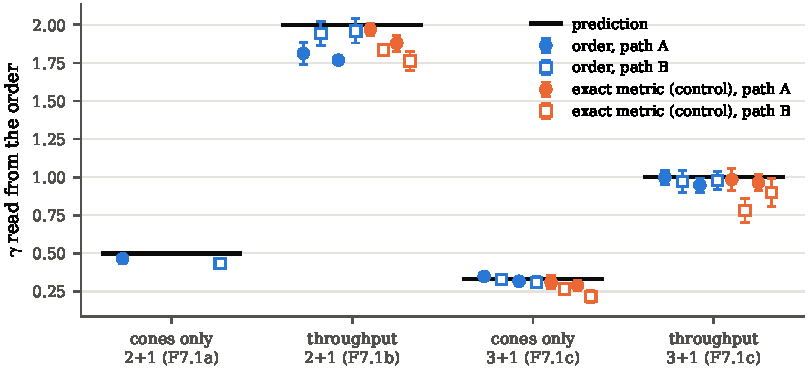
\includegraphics[width=\textwidth]{figures/fig_response.pdf}
  \caption{$\gamma$ of the responses of the order (F7.1a; F7.1b and F7.1c, two independent runs each), path A (filled) and
path B (open), against the prediction (black bar). Orange: orders sprinkled into the exact metric with the
predicted $\gamma$ and read by the same instrument in the same run (the controls of F7.1b and F7.1c); in 3+1
path B of the control reads low, which leaves F7.1c undecided. Bars: $\pm1$ standard error.}\label{fig:response}
\end{figure}

\paragraph{What this does and does not show.} The tests show that a discrete order built according
to the throughput principle has the geometry of $\gamma=1$ in 3+1. They do not show why the
substrate conserves its throughput. Part~\ref{part:geometric} answers that question at the linear
order: the principle is the linearised coupling of general relativity, and it follows from an action
of the order with the Einstein--Hilbert stiffness, which the expected Benincasa--Dowker action has.

% =============================================================================
\section{Free fall in the order}\label{sec:fall}
% =============================================================================

The order of Sec.~\ref{sec:response} carries gravity: its longest chains between two fixed events sag
towards the mass. A separate question is whether matter, moved by a local rule that reads only the
order, falls. Such a rule contains no bending law and no field; the fall has to come from inertia and from
the order itself.

\paragraph{Set-up.} The 2+1 throughput order of F7.1b with $\sigma_0=0.45$: density $e^{\sigma}$,
cones $e^{-\sigma}$, $\sigma=\sigma_0\exp(-r^2/2w^2)$, $w=8$. With the dictionary of
Sec.~\ref{sec:reading} its clock potential is $\phi=-\sigma/3$ ($\gamma=2$), which predicts the Newtonian
acceleration $a_{\rm pred}$ of a slow body. A history is continued as a longest chain: from its last event
$v$, with the event $p$ eight steps back, the rule looks at the events $q$ eight links ahead,
$L(v,q)=8$, and steps along a longest chain towards the one with the smallest $L(p,q)$, i.e.\ the
straightest continuation by the reverse triangle inequality. The reading is $R=a/a_{\rm pred}$, with $a$
from a quadratic fit of the mean radial displacement over 22 units of time. Fixed before each run: the
history falls as predicted if $\tfrac12<R\mp2\,\text{SE}<2$; in the flat order neither the histories may
drift nor the longest chains sag, and in the loaded order the longest chains must read the geometry,
$\tfrac12<R_{\max}\mp2\,\text{SE}<2$.

\paragraph{Results.}
\begin{itemize}
\item A direction carried in flat coordinates (F5.1, carried) keeps its direction and does not
  fall, $R=-0.11\pm0.04$ (the control read $R_{\max}=0.63\pm0.07$, narrowly below its band:
  \verdict{instrument failed}). A rule that keeps to the layer of the longest chains from the origin
  (F5.1, intrinsic) moves outwards, $R=-0.30\pm0.07$: \verdict{failed}.
\item The longest-chain rule started from a virtual history at rest (F5.1c) moves inwards but not with
  the Newtonian acceleration, $R=0.34\pm0.05$: \verdict{failed}. A history at rest is not a free state of
  the order.
\item The same rule started at the apex of a thrown ball (F5.1d): the history is the rising half of the
  longest chain between two events at the same place, a free state read from the order. It falls,
  $R=1.069\pm0.051$: \verdict{passed}. Flat order $R=0.15\pm0.10$; longest chains $R_{\max}=0.74\pm0.08$
  (loaded) and $0.10\pm0.12$ (flat). Fig.~\ref{fig:fall}.
\end{itemize}

\begin{figure}[t]
  \centering
  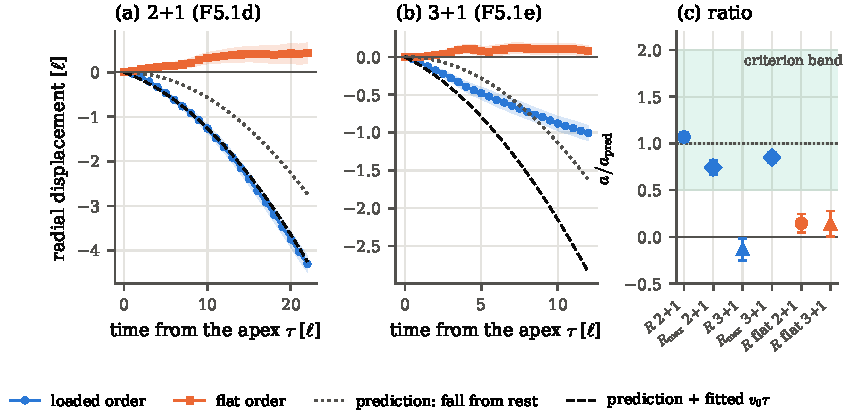
\includegraphics[width=\textwidth]{figures/fig_fall.pdf}
  \caption{Free fall from the apex (F5.1d, 2+1, 32 sprinklings per order, 40 histories each). (a) The mean
radial displacement from the apex (band $\pm1$ standard error across sprinklings) in the loaded and the flat
order; dotted: the Newtonian fall from rest at the apex radius, the prediction of the test; dashed: the same
fall with the fitted start velocity $v_0$. (b) $R=a/a_{\rm pred}$ and the control $R_{\max}$ with the
criterion band $\tfrac12<R<2$. Bars: $\pm1$ standard error.}\label{fig:fall}
\end{figure}

\paragraph{What this does and does not show.} In an order shaped by matter, a history that continues as a
longest chain falls with the Newtonian acceleration, without a bending rule, provided it starts from a
free state of the order. The limits are: one run in 2+1; the start from the apex was introduced after
F5.1c failed, with its criteria fixed before the run; the fit gives an inward start velocity
$v_0=-0.069\pm0.011$, while the rising half of the history moved outwards at $+0.026$, a jump at the apex
that the rule does not yet explain; the fall is $1.44$ times what the longest chains read of the geometry;
and the flat order drifts slightly outwards, within its tolerance. A replication, the 3+1 version and frame
dragging by a rotating source are the next tests.

% =============================================================================
\section{The Benincasa--Dowker operator and action}\label{sec:bd}
% =============================================================================

For a causal set sprinkled at density $\rho$ into a $D$-dimensional spacetime, the smeared
Benincasa--Dowker (BD) operator acting on a field $f$ is~\cite{BenincasaDowker2010,Sorkin2007,DowkerGlaser2013}
\begin{equation}\label{eq:Bdiscrete}
  (B_\epsilon f)(x)=-a_D(\epsilon\rho)^{2/D}\Big[f(x)+\sum_{y\prec x}K_\epsilon(n_{xy})\,f(y)\Big],
\end{equation}
\begin{equation}
  K_\epsilon(n)=\epsilon(1-\epsilon)^n\sum_i C_i\binom{n}{i}\Big(\frac{\epsilon}{1-\epsilon}\Big)^{i},
\end{equation}
where $n_{xy}$ is the number of elements strictly between $y$ and $x$. In 3+1 the coefficients are
$C=(-1,9,-16,8)$ and $a_4=4/\sqrt6$. Its expectation over sprinklings is
\begin{equation}\label{eq:Bexpect}
  \Ex[B_\epsilon f](x)=-a_D(\epsilon\rho)^{2/D}\Big[f(x)+\epsilon\rho\!\int_{J^-(x)}\!\!\sqrt{-g(y)}\;
    g_k\big(\epsilon\rho V(x,y)\big)f(y)\,\dd^Dy\Big],
\end{equation}
with $V(x,y)$ the proper volume of the interval and
\begin{equation}\label{eq:gk}
  g_k(w)=e^{-w}\sum_i C_i\frac{w^i}{i!}.
\end{equation}
In the continuum limit it tends to $\Box_g-\tfrac12R$ in curved
spacetime~\cite{BenincasaDowker2010,Belenchia2016}. The laboratory confirmed this limit with its own
instruments, for conformally flat geometries (K.11, K.11c) and, separately for the density part and
the cone part, for the geometry with bent light (K.13a: within $0.8$--$2.4\%$ at a field width of
$32\ell_k$).

The BD \emph{action} of a causal set is
\begin{equation}\label{eq:SBD}
  S_\BD=-\frac{2}{\rho}\sum_x (B_\epsilon 1)(x),
\end{equation}
whose expectation tends, in the continuum, to the Einstein--Hilbert action $\int\sqrt{-g}\,R$ plus
boundary terms~\cite{BuckDowkerJubbSurya2015}. In this paper the BD action is the candidate dynamics of the order. Part~\ref{part:geometric}
computes its expectation to second order in static perturbations and compares the result with the
Einstein--Hilbert value, which enters only as the normalisation of the comparison.


\part{Units, Parameters and the SI Bridge}\label{part:units}
% =============================================================================
%  Part IV -- Units, parameters and the SI bridge (catalogue of symbols)
% =============================================================================

Causal Physics is formulated at the level of causal structure, not of spacetime geometry. Its
fundamental quantities are therefore dimensionless and relational: counts of events, relations
between them and ratios of such counts. Comparison with observation nevertheless requires
quantities reported in SI units. This part states how the two are kept apart, lists the symbols of
the theory, and states which numbers are parameters and which are bridges.

% =============================================================================
\section{Three descriptive layers}\label{sec:layers}
% =============================================================================

The theory separates three layers of description. The separation is a structural requirement, not
a convenience.

\begin{center}
\begin{tabularx}{\linewidth}{lXX}
\toprule
layer & role & permitted content\\
\midrule
causal layer & physical ontology and dynamics & events, the relation $\prec$, counts of events,
  flows, response variables, the action of the order\\
bridge layer & metrology only & the discreteness scale, unit conversion, projection of counts onto
  lengths, times and accelerations\\
observational layer & empirical comparison & SI quantities, catalogues, measured accelerations,
  delays, deflections\\
\bottomrule
\end{tabularx}
\end{center}

Three rules follow. Causal variables never carry physical dimensions. Observational quantities never
take part in causal evolution. Bridge parameters never change a rule, a threshold or a weight of the
causal layer. A construction that violates any of the three reintroduces background structure and
is excluded.

Coordinates have a special status. They are not part of the causal layer. An \emph{instrument} may
use them as a declared readout, for example to place the events of a sprinkling or to report a
profile as a function of radius; a \emph{rule} of the dynamics may not (Sec.~\ref{sec:method-ax}).

% =============================================================================
\section{Catalogue of symbols}\label{sec:symbols}
% =============================================================================

For Greek letters and special symbols the middle column gives the name and the pronunciation
(International Phonetic Alphabet, English).

\newcommand{\rd}[2]{#1~\textipa{/#2/}}
\newenvironment{symtab}{\begin{center}\small\begin{tabular}{l>{\raggedright\arraybackslash}p{4.0cm}>{\raggedright\arraybackslash}p{7.4cm}}
\toprule symbol & read as & meaning\\\midrule}{\bottomrule\end{tabular}\end{center}}

\subsection{Structure of the order}

\begin{symtab}
$v,\ u,\ x,\ y$ & & events (elements of the causal set)\\
$u\prec v$ & \rd{$u$ precedes $v$}{prI"si:dz} & causal relation: $u$ can influence $v$\\
$u\prec\!\!\cdot\, v$ & \rd{link}{lINk} & link: $u\prec v$ with nothing in between\\
$I(u,v)$ & & causal interval $\{w:u\prec w\prec v\}$\\
$n(u,v)$ & & number of elements strictly inside $I(u,v)$\\
$J^-(x)$ & \rd{J minus}{dZeI "maIn@s} & causal past of $x$\\
$\rho$ & \rd{rho}{roU} & \textbf{fundamental density of the substrate}: the mean number of events per unit
  proper four-volume. In a sprinkling the number of events in a region of volume $V$ is Poisson
  distributed with mean $\rho V$. It sets the discreteness length $\ell=\rho^{-1/D}$ and, with
  $\epsilon$, the non-locality scale $\ell_k$. It is the same everywhere: near matter the
  \emph{coordinate} density changes ($\rho_c$), not $\rho$\\
$D=d_s+1$ & & spacetime dimension; $d_s$ spatial dimensions\\
$N$ & & number of events in a region\\
\end{symtab}

\subsection{Transport, matter and action}

\begin{symtab}
$F_v$ & & flow carried by event $v$ (non-negative, conserved)\\
$\Delta Q_v$ & \rd{delta}{"dElt@} $Q$ & flow stored at $v$ (the residual of the balance at $v$)\\
$s_v$ & & source term at $v$\\
$u^a$ & & four-velocity carried by a flow as its state\\
$P^a=F\,u^a$ & & four-momentum of a flow; merging rule $F=|P|$\\
$T^{ab}$ & & energy--momentum tensor of flows, Eq.~\eqref{eq:Tab}\\
$e_0$ & & rest-frame energy density of a flow ($T_{ab}u^au^b$)\\
$C$ & & capacity: the largest flow an event can pass on\\
$\sigma_v=F_v/C$ & \rd{sigma}{"sIgm@} & load of event $v$\\
$\Delta\tau$ & \rd{delta tau}{"dElt@ taU} & proper time between successive events of a flow, counted by the order\\
$S_m=-\sum m\,\Delta\tau$ & $\Sigma$: \rd{sum}{s2m} & action of a flow (Axiom~\ref{ax:action})\\
$\mathcal R=\sum_v Z_v\,\Delta\tau$ & \rd{script R}{skrIpt A:r} & Causal Resistance Functional, the impedance-weighted action\\
\end{symtab}

\subsection{Response of the substrate}

\begin{symtab}
$\Pi_v$, $0<\Pi_v\le1$ & \rd{capital pi}{"k\ae pIt@l paI} & permeability, read as the local clock rate:
  $\dd\tau=\Pi\,\dd t$ along a static world line\\
$L=\ln\Pi$ & \rd{log pi}{lAg paI} & logarithmic clock potential; the stress coordinate of the substrate
  ($L<0$ near matter)\\
$I_v\ge1$ & & stiffness: resistance of the order to reconfiguration\\
$Z_v=I_v/\Pi_v\ge1$ & & impedance\\
$c_{\rm eff}$ & \rd{c effective}{si: I"fEktIv} & local speed of the causal cone; $c_{\rm eff}=c$ in the empty substrate\\
$\rho_c$ & \rd{rho c}{roU si:} & density of events per \emph{coordinate} volume, in units of $\rho$
  ($=\sqrt{-g}$ in a sprinkling); grows near matter\\
$\rho_s$ & \rd{rho s}{roU Es} & density of saturated events: the source of the static field in the rest
  frame of the matter ($T_{ab}u^au^b$ of the flows)\\
$q=\rho_c\,c_{\rm eff}$ & & causal throughput (conserved, Sec.~\ref{sec:response})\\
\end{symtab}

\subsection{Geometry read from the order}

\begin{symtab}
$\phi$ & \rd{phi}{faI} & clock potential, read from the number of elements of a small interval at rest\\
$\psi$ & \rd{psi}{saI} & spatial potential; $\phi+\psi$ is read from the boundary of the relation and
  $\phi-d_s\psi$ from the density\\
$\gamma=\psi/\phi$ & \rd{gamma}{"g\ae m@} & post-Newtonian parameter (light deflection, Shapiro delay)\\
$\beta$ & \rd{beta}{"beIt@} & post-Newtonian parameter of the non-linearity of the clock field\\
$U$ & & Newtonian potential ($U=-\phi$ in the weak field)\\
$\eta_{ab}$ & \rd{eta}{"eIt@} & Minkowski metric\\
$h_{ab},\ \bar h_{ab}$ & \rd{h bar}{eItS bA:r} & metric perturbation and its trace-reversed form\\
$\Box_g$ & \rd{box}{bAks}, d'Alembertian & wave operator of the metric $g$\\
$R$ & & scalar curvature\\
\end{symtab}

\subsection{Operators and the action of the order}

\begin{symtab}
$\epsilon$, $0<\epsilon\le1$ & \rd{epsilon}{"Eps@lAn} & smearing parameter of the Benincasa--Dowker operator\\
$\ell_k=(\epsilon\rho)^{-1/D}$ & \rd{ell k}{El keI} & non-locality scale\\
$C_i$ & & Benincasa--Dowker coefficients; in 3+1 $(-1,9,-16,8)$, fixed by $D$\\
$a_D$ & & normalisation; $a_4=4/\sqrt6$\\
$K_\epsilon(n)$ & \rd{K epsilon}{keI "Eps@lAn} & smeared kernel, Eq.~\eqref{eq:Bdiscrete}\\
$g_k(w)$ & & expected kernel, Eq.~\eqref{eq:gk}\\
$B_\epsilon$, $\Ex[B_\epsilon]$ & \rd{expectation of B}{Ek.spEk"teIS@n} & discrete BD operator and its expectation\\
$S_\BD$ & & BD action of the order, Eq.~\eqref{eq:SBD}\\
$V(x,y)$ & & proper volume of the interval between $y$ and $x$\\
$\hat K(k,T)$ & \rd{K hat}{keI h\ae t} & ratio of the second-order BD action to its Einstein--Hilbert value
  (Sec.~\ref{sec:bdaction}); $K_{\rm loc}$ its local part\\
$c_T$ & & coefficient of the age term of the BD action\\
$\cA,\ \cB,\ \cC$ & \rd{script A, B, C}{skrIpt eI bi: si:} & coefficients of the static quadratic form of the action of
  the order: conformal, mixed and optical sector (Einstein--Hilbert $6$, $8$, $2$), Sec.~\ref{sec:mixed}\\
$T_{\rm U}$ & & Unruh temperature (Sec.~\ref{sec:jacobson}); not the age $T$\\
$T$ & & age: how long a static field has existed in the past of an event\\
$\kappa$ & \rd{kappa}{"k\ae p@} & coupling of flows to the order\\
$\hbar$ & \rd{h-bar}{eItS bA:r} & reduced Planck constant\\
$\ell_P$ & \rd{ell P}{El pi:} & Planck length\\
\end{symtab}

% =============================================================================
\section{Parameters of the theory}\label{sec:parameters}
% =============================================================================

\paragraph{Fundamental.} The causal layer has two numbers that are not fixed by the order itself:
the density $\rho$, which sets the discreteness length $\ell=\rho^{-1/D}$, and the smearing
parameter $\epsilon$, which sets the non-locality scale $\ell_k=(\epsilon\rho)^{-1/D}\ge\ell$. All
results of Part~\ref{part:geometric} are stated in units of $\ell_k$; the expectation values of the
operator and of the action depend on $\epsilon$ and $\rho$ only through the product $\epsilon\rho$.
For $\epsilon=1$, $\ell_k=\ell$.

\paragraph{Fixed by the dimension.} The coefficients $C_i$ and the normalisation $a_D$ are not
parameters: they are fixed by requiring that the expected operator reproduce the d'Alembertian in
$D$ dimensions.

\paragraph{The coupling.} The strength with which a flow acts on the order, $\kappa$, becomes
Newton's constant in the bridge layer. It is not tuned in the causal layer: in the linear regime
it fixes only the normalisation of the field, never its shape or its tensor structure.

\paragraph{Working parameters of models.} Particular models of the response of the substrate (the
saturation level of a load-driven clock law, a materialisation threshold, a feedback exponent) carry
working parameters. They are properties of a model, not constants of nature, and no result of this
paper depends on their values.

\paragraph{Laboratory units.} The laboratory works in units in which $\rho=1$, or $\epsilon\rho=1$
for computations with the expected operator; lengths are then counted in $\ell$ or $\ell_k$.

% =============================================================================
\section{The SI bridge}\label{sec:bridge}
% =============================================================================

\paragraph{The speed of light.} In a Lorentz-invariant substrate the boundary of the relation has
the same slope in every frame. Reporting that slope in SI units defines $c$; $c$ is a conversion
between the counting of events along time and across space, not an additional constant of the
causal layer.

\paragraph{Newton's constant (conditional).} The bridge to $G$ goes through the entropy of horizons
(Sec.~\ref{sec:jacobson}). If the entropy of a horizon is the number of horizon molecules times an
entropy $s_0$ per molecule, the entropy density per unit area is $\eta=s_0\,a^{(4)}/\ell^2$ with
$a^{(4)}=\sqrt3/10$, and the thermodynamic derivation of Einstein's equations gives
$G=1/(4\hbar\eta)$~\cite{Jacobson1995}. Then
\begin{equation}\label{eq:lP}
  \ell^2=4s_0\,a^{(4)}\,\ell_P^2=\frac{2\sqrt3}{5}\,s_0\,\ell_P^2,\qquad
  \ell\simeq1.075\sqrt{s_0}\;\ell_P ,
\end{equation}
with $\ell_P$ the Planck length. The discreteness length is thereby tied to $G$ up to $s_0$. This is a
relation of consistency, not a prediction of $G$: it becomes predictive only when $\ell$ or $s_0$ is
measured independently.

\paragraph{The non-locality scale.} The smearing scale $\ell_k$ is not fixed by any bridge. It is a
free scale of the theory, to be bounded or measured by the predictions of Part~\ref{part:predictions}. For
fields propagated by the non-local operator existing data give $\ell_k\lesssim10^{-19}$\,m; whether this
applies to Causal Physics is discussed in Sec.~\ref{sec:window}.

\paragraph{Projection of counts.} Within the plateau, where geometry is a reliable compression of
the order, counts are projected onto SI quantities: a number of elements $N$ of a region onto a
four-volume $N/\rho$, the length of the longest chain onto a proper time, the clock potential $L$
onto the Newtonian potential $U/c^2$. Outside the plateau the projections persist formally but lose
physical meaning.

\paragraph{No acceleration scale.} The present formulation introduces no acceleration scale in any
layer (Sec.~\ref{sec:astro-cosmo}).


\part{Axioms of Causal Physics}\label{part:axioms}
% =============================================================================
%  Part V -- Axioms of Causal Physics
% =============================================================================

This part states the foundations of Causal Physics in two groups. The \emph{methodological
principles} say how the theory may be built and tested; they are rules of inquiry and say nothing
about nature. The \emph{physical axioms} say what the world is made of and how it behaves; they are
the content of the theory. For each physical axiom we state its status: whether it is an
\emph{input} (assumed), a \emph{derived} statement, or \emph{tested} by the laboratory.

No background manifold, metric, coordinate system or spacetime dimension is assumed. All such
structures, where they exist, are read from the order.

% =============================================================================
\section{Methodological principles}\label{sec:method-ax}
% =============================================================================

\begin{definition}[M1: Causal primacy]
No geometry, coordinate system, external clock or unit enters the causal layer. Geometry is a
description of the order, read from it by declared instruments.
\end{definition}

\begin{definition}[M2: Separation of layers]
Causal, bridge and observational quantities are kept apart (Sec.~\ref{sec:layers}). Observational
quantities never act on the causal dynamics, and bridge parameters never change its rules.
\end{definition}

\begin{definition}[M3: Order and number]
Every rule of the dynamics uses only the order and counts of events, or states of events derived
from them. Coordinates may appear in an instrument as a declared readout, never in a rule.
\end{definition}

\begin{definition}[M4: Causality and covariance of rules]
The state of an event depends only on its causal past. A rule gives the same result in every
inertial frame and in every order of computation compatible with the causal order (every linear
extension).
\end{definition}

\begin{definition}[M5: Finiteness]
A rule and its results are finite and well defined without a wall of the region or a regulator. A
result that holds only because of the boundary of a simulation is a property of the simulation.
\end{definition}

\begin{definition}[M6: Input and output]
Every statement is classified as an input (postulate, tuned parameter) or an output (it followed
without being put in). A test of an output that was put in as an input proves nothing.
\end{definition}

\begin{definition}[M7: Pre-registration and falsifiability]
Every test states its question, prediction, null model and numerical criterion before it is run,
and declares the level of conclusion it can support: a \emph{calibration} establishes an instrument and
says nothing about physics; a \emph{mechanism} shows that a mechanism works in a declared model; a
\emph{chain} shows that connected mechanisms reproduce a predicted behaviour; a \emph{prediction} is an
independent result fixed in advance. No output may claim more than its level allows. A changed criterion
makes a new revision of the test, and the earlier verdict stays. A new hypothesis may follow a failure, but
it may not change the criteria by which the earlier test failed. Negative results are kept.
\end{definition}

% =============================================================================
\section{Physical axioms}\label{sec:phys-ax}
% =============================================================================

\subsection{The substrate}

\begin{axiom}[Primacy of events]\label{ax:events}
Physical reality consists of elementary events. An event is an irreducible act of realisation, not a
persisting entity. It has no intrinsic position, duration, mass, energy, charge or scale. All
physical attributes are relational: they are patterns of causal connectivity among events.
\end{axiom}
\begin{status} Input. \end{status}

\begin{axiom}[Causal order]\label{ax:order}
Causal relations form a partial order: they are transitive and acyclic, and every interval contains
finitely many events. Closed causal loops do not exist. Time is the order itself; there is no
external time and no global simultaneity.
\end{axiom}
\begin{status} Input. The structure is a causal set. \end{status}

\begin{axiom}[Lorentz-invariant substrate]\label{ax:substrate}
On the plateau the order is, statistically, a uniform sprinkling of a Lorentzian manifold at density
$\rho$: the number of events in a region is $\rho$ times its proper volume, and no frame is
preferred. Dimension, distance and duration are read from order and number alone.
\end{axiom}
\begin{status} Input, supported by tests: the degree of an event is not bounded (F0.3), local
growth rules with bounded degree produce no manifold-like order (F6.1, F6.2), and geometry is read
blindly from the order (K.1, K.3, K.16b, K.16c). \end{status}

\subsection{Transport and matter}

\begin{axiom}[Causal continuity]\label{ax:continuity}
Influence is transported along the relations of the order and is conserved at every event:
\begin{equation}
  \sum_{\text{in}}F+s_v=\sum_{\text{out}}F+\Delta Q_v .
\end{equation}
What enters an event leaves it or is stored there.
\end{axiom}
\begin{status} Input. Tested consequence: Gauss's law for a steady source, $J/S=1.003$--$1.004$ in
2+1 and 3+1 (F1.1). \end{status}

\begin{axiom}[Finite capacity]\label{ax:capacity}
The flow an event can pass on is bounded by a capacity $C$. Capacity limits the flow through an
event, not the number of its relations.
\end{axiom}
\begin{status} Input. Supported by F1.8 (not yet robust to the seed). \end{status}

\begin{axiom}[Flows carry momentum]\label{ax:momentum}
A flow carries its four-velocity $u^a$ as a state passed from event to event. When flows merge, the
merged flow is the length of the summed four-momentum, $F=|\sum P|$, so that four-momentum is
conserved. The flows then have an energy--momentum tensor $T^{ab}$, Eq.~\eqref{eq:Tab}.
\end{axiom}
\begin{status} Input. Tested consequences: a flow with a carried direction is localised and moves with
its source, i.e.\ has inertia (F3.6, replicated); $T^{ab}$ is measured correctly for dust,
counter-streaming beams and an isotropic gas, and the merging rule conserves four-momentum exactly
(K.15, replicated). \end{status}

\subsection{Response and action}

\begin{axiom}[Local response]\label{ax:response}
Every event has a response variable $\Pi_v$, $0<\Pi_v\le1$, read as its clock rate, and a stiffness
$I_v\ge1$; its impedance is $Z_v=I_v/\Pi_v$. The axiom does not fix how $\Pi_v$ depends on the
load, on the surrounding order or on other causal variables; that dependence is a separate,
independently testable law of response.
\end{axiom}
\begin{status} Input. The law of response is not part of the axiom. In the linear regime it is
fixed by the dynamics of the order (Axiom~\ref{ax:dynamics}, Part~\ref{part:geometric}). \end{status}

\begin{axiom}[Action of a flow]\label{ax:action}
The action of a flow is its proper time counted by the order,
\begin{equation}
  S_m=-\sum m\,\Delta\tau ,
\end{equation}
where $\Delta\tau$ is the proper time between successive events of the flow, as given by the length
of the longest chain or by the number of elements of a small interval. The Causal Resistance
Functional $\mathcal R=\sum_v Z_v\Delta\tau$ is its impedance-weighted form.
\end{axiom}
\begin{status} Input. Derived consequences: on a fixed order the motion is geodesic in the conformal
geometry $\Pi^2\eta$ (tested: F2.2, F2.4, F2.5); the coupling of a flow to the order is
$\delta S_m/\delta h_{ab}=\tfrac12T^{ab}$, i.e.\ through the rest frame of the flow, and contributions
of different flows add (Sec.~\ref{sec:action}). How the weight $Z_v$ relates to the response of the
order beyond the linear regime is open. \end{status}

\subsection{Dynamics of the order}

\begin{axiom}[The order responds to matter]\label{ax:dynamics}
The order is dynamical. Its configurations are weighted by an action of the order, and matter
changes the order: near flows, causal cones narrow and events are added. Causality itself is
preserved (Axioms~\ref{ax:order} and~\ref{ax:continuity}). The candidate action of the order is the
Benincasa--Dowker action $S_\BD$ (Sec.~\ref{sec:bd}).
\end{axiom}
\begin{status} Input (that the order is dynamical and which action weights it). Derived and computed
consequences:
\begin{itemize}
\item the expected BD action has the Einstein--Hilbert stiffness in the static conformal sector,
  $6.0003$ against $6$ (F6.8a), in the mixed sector, $7.983$ against $8$ (F6.8b2), and in the optical sector,
  $2.002$ against $2$ (F6.8c2); with Axiom~\ref{ax:action} the linear response of the order is then
  the coupling of linearised general relativity to $T_{ab}$ (Part~\ref{part:geometric});
\item in 3+1 this response is the conservation of causal throughput, $\rho_c\,c_{\rm eff}=\text{const}$,
  which gives $\gamma=1$ (tested on discrete orders: F7.1c, raw $\gamma=1.000\pm0.045$, formal verdict
  undecided);
\item a substrate rule realising it makes pressure and motion gravitate and drags the cones
  (tested: F7.4a).
\end{itemize}
How the order grows (a sequential growth law or a sum over orders weighted by $S_\BD$) is
open. \end{status}

% =============================================================================
\section{What is derived, and from what}\label{sec:ax-summary}
% =============================================================================

\begin{center}
\begin{tabularx}{\linewidth}{>{\raggedright\arraybackslash}X>{\raggedright\arraybackslash}p{2.6cm}>{\raggedright\arraybackslash}p{4.8cm}}
\toprule
statement & from & status\\
\midrule
time as order, no global simultaneity & Ax.~\ref{ax:order} & derived\\
geometry read from order and number & Ax.~\ref{ax:substrate} & tested (K.16b/c)\\
Gauss's law & Ax.~\ref{ax:continuity} & tested (F1.1)\\
inertia of localised matter & Ax.~\ref{ax:momentum} & tested (F3.6)\\
conservation of four-momentum in merging & Ax.~\ref{ax:momentum} & tested (K.15)\\
geodesic motion & Ax.~\ref{ax:action} & tested (F2)\\
coupling through $T_{ab}$ in the rest frame of each flow & Ax.~\ref{ax:action} & derived\\
Einstein--Hilbert stiffness of the order & Ax.~\ref{ax:dynamics} & computed, all three sectors (F6.8a, F6.8b2, F6.8c2)\\
throughput principle, $\gamma=1$ in 3+1 & Ax.~\ref{ax:action}, \ref{ax:dynamics} & derived; F7.1c\\
tensor coupling, frame dragging & Ax.~\ref{ax:action}, \ref{ax:dynamics} & derived; F7.4a\\
non-linear completion by general relativity & Ax.~\ref{ax:dynamics} + uniqueness & derived (programme)\\
\bottomrule
\end{tabularx}
\end{center}


\part{The Geometric Limit: Gravity from the Response of the Order}\label{part:geometric}
% =============================================================================
%  Part VI -- The geometric limit: gravity from the response of the order
% =============================================================================

This part derives and tests the gravitational coupling of Causal Physics in the regime where
geometry is a reliable description of the order. It proceeds in five steps: what the coupling must
look like (Sec.~\ref{sec:tensor}), a substrate rule that realises it on causal sets
(Sec.~\ref{sec:rule}), why the rule follows from the action of the order (Sec.~\ref{sec:fromaction}),
a direct computation of that action to second order (Sec.~\ref{sec:bdaction}), and the static
propagator that turns the result into predictions (Sec.~\ref{sec:propagator}). The static section of
the field to first post-Newtonian order (Sec.~\ref{sec:static}) and the thermodynamic completion
beyond the linear order (Sec.~\ref{sec:jacobson}) close the part.

Conventions: signature $(-,+,+,+)$, $c=1$, $g=\eta+h$, $\bar h_{ab}=h_{ab}-\tfrac12\eta_{ab}h$. A static
weak field has $h_{00}=2U$, $h_{ij}=2\gamma U\delta_{ij}$, with $U>0$ the Newtonian potential and $u^a$
the four-velocity of the source.

% =============================================================================
\section{What the coupling must look like}\label{sec:tensor}
% =============================================================================

\subsection{The parameter \texorpdfstring{$\gamma$}{gamma} is a ratio of two couplings}

In the rest frame of a dust source, a static weak field with parameter $\gamma$ in $d_s$ spatial
dimensions has
\begin{equation}
  \bar h_{00}=U(1+\gamma d_s),\qquad \bar h_{ij}=U(1+2\gamma-\gamma d_s)\,\delta_{ij}.
\end{equation}
In 3+1 this is
\begin{equation}\label{eq:hbar-gamma}
  \bar h_{ab}=U\big[(1-\gamma)\,\eta_{ab}+2(1+\gamma)\,u_au_b\big].
\end{equation}
The field is a mixture of two couplings: to the trace of the energy--momentum tensor ($\eta_{ab}$) and
to the tensor itself ($u_au_b$).
\begin{itemize}
\item $\gamma=-1$: $\bar h_{ab}=2U\eta_{ab}$, pure trace coupling (spin 0, Nordstr\"om). Light is not
  deflected and does not gravitate, because the electromagnetic field has zero trace. This is the
  geometry of a fixed order (Sec.~\ref{sec:action}).
\item $\gamma=1$: $\bar h_{ab}=4U\,u_au_b$, pure coupling to $T_{ab}=\rho\,u_au_b$ with no trace part.
  This is linearised general relativity, $\Box\bar h_{ab}=-16\pi G\,T_{ab}$.
\item $\gamma=1/3$ (cones that only narrow) is a mixture of the two.
\end{itemize}

\subsection{The throughput principle is the tensor coupling}

The throughput principle $\rho_c\,c_{\rm eff}=\text{const}$ (Sec.~\ref{sec:response}) gives
$\gamma=2/(d_s-1)$. Pure tensor coupling of dust ($\bar h_{ij}=0$) gives $\gamma=1/(d_s-2)$. The two
coincide only for $d_s=3$. In three spatial dimensions, therefore, the throughput principle \emph{is}
the coupling of linearised general relativity: the deformation of the order lies only along the flow
($u_au_b$) and vanishes across it. Three consequences follow at once:
\begin{itemize}
\item light gravitates, and pressure gravitates as $\rho+3p$;
\item a moving source produces $g_{0i}$: inertial frames are dragged;
\item the field of many flows is a sum over flows, $\bar h_{ab}\propto\sum F\,u_au_b\,G_{\rm ret}$, whose
  transverse traceless part is a gravitational wave with the two polarisations $+$ and $\times$.
\end{itemize}

\subsection{A scalar field cannot be the whole law}

A single scalar clock field $\Pi$ in a fixed frame satisfies the static weak-field tests if the metric
is chosen with $\gamma=1$, but it cannot be the complete law of gravity. It has no $g_{0i}$, so it
cannot reproduce the frame dragging measured by Gravity Probe~B~\cite{Everitt2011}. Normalised to
Newton's law, a scalar field radiates quadrupole power
$P=\tfrac{G}{60}\big[(\mathrm{tr}\,\dddot I)^2+2\,\dddot I_{ij}\dddot I_{ij}\big]$, which for a circular
binary is exactly $1/6$ of the general relativistic value; binary pulsars agree with general relativity
to $10^{-3}$--$10^{-4}$~\cite{Kramer2021}. A scalar field is therefore the static section of the field in the rest frame
of its source, not the field itself (Sec.~\ref{sec:static}).

% =============================================================================
\section{The substrate rule and its test}\label{sec:rule}
% =============================================================================

\subsection{The rule}

The coupling of Sec.~\ref{sec:tensor} requires the order to know in which frame each flow is at rest.
The flows carry this information (Axiom~\ref{ax:momentum}). The substrate rule is:
\begin{enumerate}
\item \emph{own frame}: every flow narrows the causal cone in its own rest frame;
\item \emph{additivity}: flows that load the same relation share its capacity, and their cone deficits
  add;
\item \emph{throughput}: the density of events rises by $e^{\sigma_{\rm tot}}$, with $\sigma_i$ the
  rest-frame load of flow $i$ and $\sigma_{\rm tot}=\sum_i\sigma_i$.
\end{enumerate}
For a candidate relation with separation $d^a$ from an event loaded by flows with four-velocities
$u_i$, the relation is kept if and only if
\begin{equation}\label{eq:rule}
  d^0>0,\qquad -d_0^2+|\vec d|^2+\sum_i a_i\,(u_i\!\cdot d)^2\le0,\qquad
  a_i=\frac{\sigma_i}{\sigma_{\rm tot}}\big(1-e^{-2\sigma_{\rm tot}}\big).
\end{equation}
For flows at rest this is the single-flow throughput rule with cones narrowed to $e^{-\sigma_{\rm tot}}$.
The order is built from a flat sprinkling by keeping or discarding relations event by event; no metric
is sprinkled, and no field equation, Green function or trace reversal enters.

\subsection{The test: counter-streaming flows}

Two equally strong flows moving at $+v$ and $-v$ have zero momentum density but non-zero energy and
spatial stress. The candidate rules therefore predict different clock fields. With the rest-frame load
of each flow fixed, the amplitude of the clock field relative to $v=0$ is predicted to be:
\begin{center}
\begin{tabular}{lcc}
\toprule
rule & linear prediction & at $v=0.6$\\
\midrule
tensor rule \eqref{eq:rule} & $\Gamma_v^2(1+v^2)$ & $2.125$ (exact, non-linear: $2.361$)\\
energy density in the mean-flow frame & $\Gamma_v^2$ & $1.5625$\\
laboratory-frame density & $\Gamma_v$ & $1.25$\\
rest density (event count) & $1$ & $1$\\
\bottomrule
\end{tabular}
\end{center}
($\Gamma_v=1/\sqrt{1-v^2}$.) The amplitude is read in the near field, transverse to uniform flows, because
for a compact stationary system the stress integrates to zero (von Laue) and the $1/r$ tail cannot
distinguish the rules.

\paragraph{Result} (F7.4a, 3+1, 16 sprinklings per configuration, $\sim5.6\times10^4$ events,
\verdict{passed}). The blind instrument reads:
\begin{itemize}
\item amplitude ratio $R=A(0.6)/A(0)=2.401\pm0.053$ against $2.361$ for the tensor rule; the energy
  density reading ($1.5625$) is $16$ standard errors away. Pressure gravitates, not only energy;
\item cone anisotropy along/across the flows $K=1.221\pm0.012$ against $1.192$; every scalar rule of the
  mean-flow frame gives exactly $1$;
\item a single flow at $0.6c$ (reported): $R=2.538$ against $2.519$; the cone tilts, with a deficit
  against the flow $17.6$ times the deficit along it (prediction $12$, scalar rules $1$). The order drags
  its cones with the flow. The downstream deficit matches exactly ($-0.065$ against $-0.065$).
\end{itemize}
The flat control reads zero, and an isotropic order reads isotropic ($K=1.002\pm0.004$)
(Fig.~\ref{fig:counter}).

\begin{figure}[t]
  \centering
  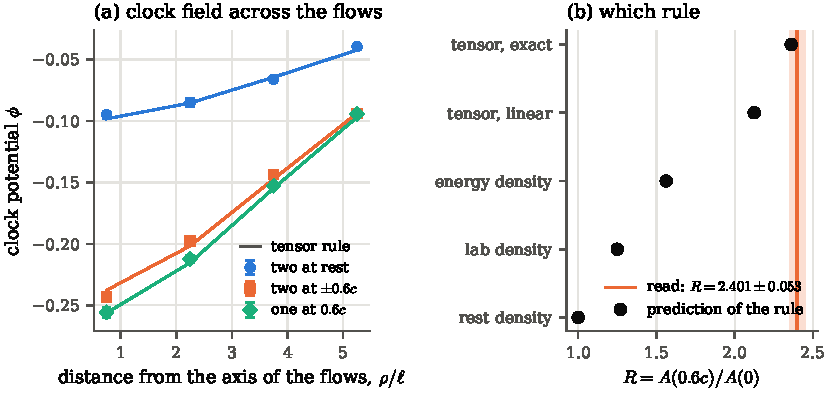
\includegraphics[width=\textwidth]{figures/fig_counter.pdf}
  \caption{Counter-streaming flows (F7.4a, 3+1, 16 sprinklings per configuration). (a) The clock potential read across the
flows (points, $\pm1$ standard error) against the tensor rule (lines) for two flows at rest, two flows at
$\pm0.6c$ and one flow at $0.6c$. (b) The amplitude ratio $R=A(0.6c)/A(0)$ read (orange line, band $\pm1$
standard error) against the prediction of each candidate rule.}\label{fig:counter}
\end{figure}

The test shows that a substrate with this rule couples to $T_{ab}$ as general relativity does at the
linear order, including frame dragging, with the tensor structure arising from the response of the order
alone. The rule itself is an input. The next section shows that it is not an independent one.

% =============================================================================
\section{The rule from the action of the order}\label{sec:fromaction}
% =============================================================================

\subsection{The matter side}

By Axiom~\ref{ax:action} the action of a flow is its proper time counted by the order. For $g=\eta+h$,
\begin{equation}
  \frac{\delta S_m}{\delta h_{ab}}=\tfrac12\,T^{ab}.
\end{equation}
Two parts of the substrate rule follow without any knowledge of the dynamics of the order:
\begin{itemize}
\item \emph{own frame}: the order sees a flow only through $u^au^b$, i.e.\ in the frame in which its
  proper time is measured;
\item \emph{additivity}: the action is a sum over flows, so at the linear order their contributions add.
\end{itemize}

\subsection{One number is left}

A linear, local and Lorentz-invariant response $h_{ab}=G*T$ has two channels, $T_{ab}$ and $\eta_{ab}T$.
For static dust this is the one-parameter family \eqref{eq:hbar-gamma}: the structure of the rule is
forced up to $\gamma$. The number $\gamma$ is fixed by the action of the order. For a general static
quadratic action coupled to dust,
\begin{equation}
  \mathcal L=c_{\Phi\Phi}|\nabla\Phi|^2+c_{\Phi\Psi}\nabla\Phi\cdot\nabla\Psi+c_{\Psi\Psi}|\nabla\Psi|^2
  -\kappa'\rho\,\Phi ,
\end{equation}
with $\dd s^2=-(1+2\Phi)\dd t^2+(1-2\Psi)\dd\vec x^2$, the variation with respect to $\Psi$ gives
\begin{equation}
  \gamma=\frac{\Psi}{\Phi}=-\frac{c_{\Phi\Psi}}{2\,c_{\Psi\Psi}},
\end{equation}
independently of $c_{\Phi\Phi}$. The Einstein--Hilbert action gives (computed symbolically for $d=2,3,4$)
\begin{equation}
  c_{\Phi\Phi}=0,\qquad c_{\Phi\Psi}=-2(d-1),\qquad c_{\Psi\Psi}=(d-1)(d-2)\quad\Rightarrow\quad
  \gamma=\frac{1}{d-2},
\end{equation}
which is $\gamma=1$ in 3+1. Two remarks:
\begin{itemize}
\item $c_{\Phi\Phi}=0$: clocks have no stiffness of their own; the time part of the field is fixed by
  the spatial part and the source.
\item The throughput principle is a consequence: dust has no stress and the order has the
  Einstein--Hilbert stiffness, so the trace-reversed spatial deformation vanishes.
\end{itemize}

\subsection{The chain}

With the Benincasa--Dowker action as the dynamics of the order (Axiom~\ref{ax:dynamics}):
\begin{equation*}
  \begin{gathered}
  \text{proper time counted by the order} \;+\; \text{BD action of the order}\\
  \Longrightarrow\;\text{the substrate rule at the linear order } (\gamma=1),
  \end{gathered}
\end{equation*}
provided the BD action has the Einstein--Hilbert stiffness. It is known that the expectation of the BD
action tends to the Einstein--Hilbert action, with a boundary term, in the continuum
limit~\cite{BenincasaDowker2010,MachetWang2020}.
The quantity that matters here, however, is the static quadratic form of the \emph{discrete} action at a
finite non-locality scale, including the contributions of long, nearly null intervals. The next section
computes it.

% =============================================================================
\section{The Benincasa--Dowker action to second order}\label{sec:bdaction}
% =============================================================================

\subsection{Sectors}

Write a static metric as $g=\Omega^2[-\dd t^2+n^2\dd\vec x^2]$ with $\omega=\ln\Omega$ and $\nu=\ln n$. The
conformal factor $\omega$ does not change the causal order, only the density of events; the optical
index $\nu$ changes the light cones. For plane waves $\omega=a\cos kz$, $\nu=b\cos kz$ the
Einstein--Hilbert action, averaged over a period, is (symbolic computation)
\begin{equation}\label{eq:EHquad}
  \Big\langle\sqrt{-g}\,R\Big\rangle=\frac{k^2}{2}\,\big(6a^2+8ab+2b^2\big)+O(a^3,b^3).
\end{equation}
Matter couples only to $\omega=\Phi$; in these variables $\gamma=-1+\cB/(2\cC)$ with $\cB=8$, $\cC=2$. We compute
here the conformal coefficient, $6$ in Einstein--Hilbert, which is an exact quadrature because the order
is unchanged.

\subsection{Method}

For $g=e^{2af}\eta$ with static $f$, the expected action per unit time and volume in the bulk of a region
of age $T$ (the past of every event cut at time $T$) is
\begin{equation}
  \Ex[S]=-2\big\langle\sqrt{-g}\;\Ex[B_\epsilon1](x)\big\rangle,
\end{equation}
with $\Ex[B_\epsilon1]$ from Eq.~\eqref{eq:Bexpect}. The proper volume of an interval is the flat
volume times the average of $e^{4af}$ over the interval. The second derivative with respect to $a$ at
$a=0$ is taken analytically under the integral: with $P=e^{4af}$, $\langle\cdot\rangle$ the average over the
interval, $g_1=w\,g_k'(w)$ and $g_2=w^2g_k''(w)$,
\begin{equation}
  \frac{\partial^2}{\partial a^2}\Big[P_xP_y\,g_k\big(w\langle P\rangle\big)\Big]_{a=0}
  =16\Big[(f_x+f_y)^2g_k+2(f_x+f_y)\langle f\rangle g_1+\langle f\rangle^2g_2+\langle f^2\rangle g_1\Big].
\end{equation}
The field is a static plane wave $f=\cos kz$, averaged over its phase in closed form, so that no wall
and no slowly converging tails enter. The averages of a plane wave over a causal interval are the
Fourier transform of the 3+1 causal diamond, which we use in closed form: in the rest frame of the
interval, with half-height $h$ and four-momentum $(\omega',q')$,
\begin{equation}
  F(\omega',q')=\frac{2}{V}\int_0^h\cos\big(\omega'(h-u)\big)\,
  \frac{4\pi\,(\sin q'u-q'u\cos q'u)}{q'^3}\,\dd u ,\qquad V=\frac{2\pi h^4}{3},
\end{equation}
evaluated stably for nearly null momenta. Lengths are in units of $\ell_k$ ($\epsilon\rho=1$); the
expectation depends on $\epsilon$ and $\rho$ only through their product. The result is reported as
\begin{equation}
  \hat K(k,T)=\frac{\partial_a^2\Ex[S]}{\text{Einstein--Hilbert value }6k^2}.
\end{equation}
The Einstein--Hilbert number enters only this normalisation.

\paragraph{Instruments} (all within tolerance): the closed-form transform agrees with an independent
quadrature of the diamond to $7\times10^{-8}$; the analytic second derivative agrees with finite
differences of the curved operator to $3\times10^{-4}$; a constant conformal factor gives zero response
to $5\times10^{-5}$ of the signal; doubling every quadrature parameter changes $\hat K$ by at most
$3\times10^{-5}$.

\subsection{Results}

For every wavenumber the response is linear in the age $T$ (residuals $\le10^{-3}$), so that
\begin{equation}\label{eq:Khat}
  \hat K(k,T)=K_{\rm loc}(k)-c_T\,k^3\,T .
\end{equation}

\begin{center}
\begin{tabular}{ccccccccccc}
\toprule
$k\ell_k$ & 0.025 & 0.035 & 0.05 & 0.07 & 0.1 & 0.14 & 0.2 & 0.3 & 0.5\\
\midrule
$K_{\rm loc}$ & 0.9904 & 0.9826 & 0.9680 & 0.9438 & 0.8994 & 0.8287 & 0.7056 & 0.4687 & $-0.015$\\
\bottomrule
\end{tabular}
\end{center}

\paragraph{The local part.} A fit $K_{\rm loc}=K_0-k^2[c_1\ln(1/k)+c_0]$ over $k\ell_k\le0.1$ gives
\begin{equation}
  K_0=1.00005,\qquad c_1=3.98,\qquad c_0=0.91,\qquad\text{rms }2.3\times10^{-5}.
\end{equation}
The conformal stiffness of the discrete BD action is therefore $6K_0=6.0003$: \emph{the Einstein--Hilbert
value emerges from the counting of intervals} (F6.8a, \verdict{passed}). The discreteness corrects it
non-analytically,
\begin{equation}
  1-K_{\rm loc}\simeq(k\ell_k)^2\big[4.0\ln(1/k\ell_k)+0.9\big],
\end{equation}
and the stiffness changes sign at $k\ell_k\simeq0.49$, a wavelength of $12.7\,\ell_k$. The momentum-space form
factor of the continuum non-local d'Alembertian is known in closed form~\cite{AslanbeigiSaravaniSorkin2014,
BelenchiaBenincasaLiberati2015}; a quantitative comparison of its infrared expansion with the non-analytic
correction found here is a planned independent check.

\paragraph{The age term.} The second term of Eq.~\eqref{eq:Khat} is not local: the static response
weakens in proportion to how long the field has existed. We predicted it before computing it. A long,
nearly null interval running perpendicular to $\vec k$ stays in phase with the field over its whole length.
Expanding its contribution in the proper time $\tau$ of the interval, the moment conditions of the BD kernel,
$\int u^{p}g_k(u)\,\dd u=0$ for $p=-\tfrac12,0,\tfrac12$, remove the orders $\tau^0$, $\tau^2$ and
$\tau^4$, but not $\tau^6$. Each unit length of history therefore adds a contribution of order $k^5$,
which is $k^3T$ relative to $k^2$. In the limit of long intervals the contribution depends only on the phase
$\phi=kL\cos\theta$ and on $k\tau$, and the coefficient is a two-dimensional integral of the diamond
transform,
\begin{equation}
  \frac{\dd J}{\dd T}=\frac{2\pi}{k}\int\dd\phi\int\tau\,\dd\tau\,
  \Big[2\cos\tfrac{\phi}{2}\,F\,g_1+\tfrac12F^2g_2\Big],
\end{equation}
which gives $c_T=0.1012$--$0.1022$ for $k\ell_k=0.05$--$0.2$. The full computation gives
$c_T=0.1035\pm0.0003$ for $k\ell_k\le0.2$ and $0.098$--$0.104$ over the whole range: agreement to $2\%$,
the rest being the finite age. In physical units the relative size of the age term is
\begin{equation}
  0.1\,(k\ell_k)^3\,\frac{T}{\ell_k}=0.1\,k^3\ell_k^2\,T .
\end{equation}
Figure~\ref{fig:conformal} shows the local part with its fit and the collapse of the age term.

\begin{figure}[t]
  \centering
  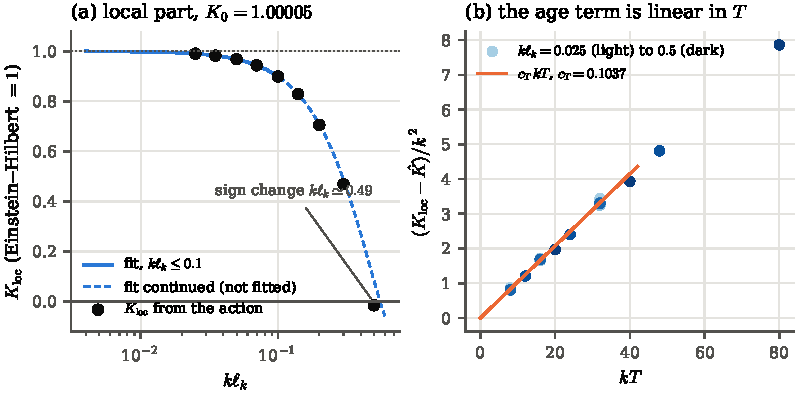
\includegraphics[width=\textwidth]{figures/fig_conformal.pdf}
  \caption{The conformal sector (F6.8a). (a) The local part $K_{\rm loc}$ of the stiffness in units of the
Einstein--Hilbert value (points), the fit $K_0-k^2[c_1\ln(1/k)+c_0]$ over $k\ell_k\le0.1$ (solid) and its
continuation (dashed), which the points beyond the fitted range follow to the sign change at
$k\ell_k\simeq0.49$. (b) The age term: $(K_{\rm loc}-\hat K)/k^2$ for every computed age and wavenumber (light to
dark: $k\ell_k=0.025$ to $0.5$) against $kT$, with the line $c_T\,kT$, $c_T$ the mean of the per-$k$ slopes over
$0.05\le k\ell_k\le0.2$. The two largest wavenumbers leave the line at large $kT$.}\label{fig:conformal}
\end{figure}

% =============================================================================
\section{Covariance and the static propagator}\label{sec:propagator}
% =============================================================================

\subsection{Form factors}

The expected BD action depends only on the geometry; it is exactly invariant under diffeomorphisms. If its
quadratic part around flat space is also covariant, it has the form
\begin{equation}
  S_2=\int\sqrt{-g}\,\Big[R+R\,F_0(\Box)\,R+C_{abcd}\,F_2(\Box)\,C^{abcd}\Big],
\end{equation}
the basis $\{R^2,C^2\}$ being complete at this order. For the plane waves of Eq.~\eqref{eq:EHquad},
$R^{(1)}=2k^2(3a+2b)\cos kz$ and $C^{(1)}\!\cdot C^{(1)}=\tfrac43\,b^2k^4\cos^2kz$: the Weyl tensor comes from
the optical index alone. Per $k^2/2$ the three coefficients become
\begin{equation}
  \cA=6+9\varphi_0,\qquad \cB=8+12\varphi_0,\qquad \cC=2+4\varphi_0+\varphi_2,\qquad
  \varphi_0=4k^2F_0,\quad \varphi_2=\tfrac43k^2F_2 .
\end{equation}

\subsection{The field of a point mass}

Matter couples to $\omega=\Phi$. Solving the quadratic form with a source gives the standard decomposition
into spin~2 and spin~0:
\begin{align}
  \frac{\Phi}{\Phi_{\rm GR}}&=\tfrac43S_2(k)-\tfrac13S_0(k), &
  \frac{\Psi}{\Psi_{\rm GR}}&=\tfrac23S_2(k)+\tfrac13S_0(k), &
  \gamma(k)&=\frac{2S_2+S_0}{4S_2-S_0},
\end{align}
with $S_0=1/(1+\tfrac32\varphi_0)$ and $S_2=1/(1-\tfrac32\varphi_2)$. Since $1+\tfrac32\varphi_0=\cA/6=\hat K$,
\emph{the computation of Sec.~\ref{sec:bdaction} determines the whole spin-0 channel}:
\begin{equation}
  S_0(k)=\frac{1}{\hat K(k,T)}=\frac{1}{K_{\rm loc}(k)-c_T\,k^3T}.
\end{equation}
The spin-0 propagator has a static pole where $\hat K=0$: at $k\ell_k\simeq0.49$ without the age term, and
with it at the length scale $(0.1\,\ell_k^2T)^{1/3}$.

These expressions assume that the quadratic action is covariant at every $k$. Section~\ref{sec:mixed}
tests this assumption directly.

\subsection{The mixed sector}\label{sec:mixed}

Covariance makes a sharp prediction without a free parameter: the mixed coefficient follows the
conformal one, $\cB/8=\cA/6=\hat K$ at every $k$. We computed $\cB$ directly (F6.8b2), for
$g=e^{2af}\big(-\dd t^2+e^{2bh}\dd\vec x^2\big)$ with $f=h=\cos kz$, phase-averaged.

\paragraph{Method.} The optical index changes the order. To first order in $b$, $y$ precedes $x$ if and
only if their time separation exceeds the optical length of the straight segment between them; by
Fermat's principle the change of the path is of second order. The past of $x$ is parametrised on the
unperturbed cone. The volume of an interval is the integral, over the spatial projection of the diamond
(a prolate spheroid, integrated in prolate spheroidal coordinates), of the time extent left by the
optical delays; the difference between the delay along the full segment and along the broken path is
formed pointwise, before averaging, so that thin intervals lose no digits. The age cut depends on $b$ and
contributes a boundary term, integrated on its own quadrature. The derivative $\partial_a\partial_b$ is
taken analytically, and the conformal $\hat K$ is computed on the same nodes and ages. The result is
reported as $\hat K_{ab}=\partial_a\partial_b\Ex[S]/(\text{Einstein--Hilbert value }4k^2)$.

\paragraph{Instruments} (all within tolerance): the derivatives of the interval volume agree with an
independent quadrature in spherical coordinates to $3.5\times10^{-5}$ and $5.8\times10^{-5}$; a uniform
optical index, a constant rescaling of space, changes no proper volume, to $9\times10^{-14}$; the
conformal $\hat K$ on this grid reproduces Sec.~\ref{sec:bdaction} to $2\times10^{-10}$; a constant
perturbation ($k=0$) gives zero response to $2.6\times10^{-4}$ in units of $\hat K$ at the smallest $k$,
for ages up to $T=320\,\ell_k$; doubling every quadrature parameter changes $\hat K_{ab}$ by at most
$3.2\times10^{-5}$.

\paragraph{Results.} For each $k$ the ages are $T=8,12,16$ times $1/k$ (at least $40\,\ell_k$), and
$\hat K_{ab}(k,T)=K_{{\rm loc},ab}(k)-c_{T,ab}\,k^3T$ is fitted as in Eq.~\eqref{eq:Khat}:
\begin{center}
\begin{tabular}{lccccc}
\toprule
$k\ell_k$ & 0.05 & 0.07 & 0.1 & 0.14 & 0.2\\
\midrule
$K_{{\rm loc},ab}$ (mixed) & 0.9683 & 0.9464 & 0.9045 & 0.8387 & 0.7261\\
$K_{\rm loc}$ (conformal, same ages) & 0.9681 & 0.9441 & 0.8999 & 0.8297 & 0.7076\\
$\Delta=K_{{\rm loc},ab}-K_{\rm loc}$ & 0.0002 & 0.0023 & 0.0046 & 0.0091 & 0.0184\\
$c_{T,ab}$ (mixed) & 0.155 & 0.197 & 0.195 & 0.195 & 0.195\\
$c_T$ (conformal) & 0.110 & 0.110 & 0.110 & 0.110 & 0.109\\
\bottomrule
\end{tabular}
\end{center}

\paragraph{The local part is covariant.} Over $k\ell_k\le0.1$ the largest difference is
$|\Delta|=4.6\times10^{-3}$, within the criterion fixed before the run ($\le10^{-2}$; F6.8b2,
\verdict{passed}). A fit $K_{{\rm loc},ab}=K_{0,ab}-k^2[c_1\ln(1/k)+c_0]$ over $k\ell_k\le0.14$ gives
$K_{0,ab}=0.9979$, i.e.\ a mixed stiffness
\begin{equation}
  \cB(k\to0)=8K_{0,ab}=7.983\qquad(\text{Einstein--Hilbert }8).
\end{equation}
Two of the three coefficients of the Einstein--Hilbert quadratic form, $6$ and $8$, therefore emerge from
the counting of intervals, and at leading order they stand in the covariant ratio.

\paragraph{Beyond the leading order the sectors differ.} For $k\ell_k=0.07$--$0.2$ the difference is a clean
analytic term,
\begin{equation}
  \Delta\simeq0.46\,(k\ell_k)^2\qquad(\Delta/k^2=0.475,\;0.462,\;0.462,\;0.461),
\end{equation}
and the age term of the mixed sector is $1.78$ times that of the conformal one ($c_{T,ab}\simeq0.195$ against
$0.110$). Neither is possible for a covariant quadratic action, local or not, which gives $\cB/8=\cA/6$ at every
$k$. The expected BD action is exactly diffeomorphism invariant, but a static field cut at age $T$ is not
a covariant configuration: the cut defines the rest frame of the field. Both differences may therefore
come from the cut rather than from the action; which of the two is open. The smallest wavenumber,
$k\ell_k=0.05$, has the longest ages of the grid and departs from both regularities
($\Delta=1.6\times10^{-4}$, $c_{T,ab}=0.155$); it is reported and not interpreted.

\paragraph{The field without assuming covariance.} Matter does not couple to $\nu$. Eliminating $\nu$
from the quadratic form $\cA\omega^2+\cB\omega\nu+\cC\nu^2$ gives $\nu=-\cB\omega/(2\cC)$, and therefore
\begin{equation}\label{eq:gammaABC}
  \gamma(k,T)=\frac{\cB}{2\cC}-1,\qquad
  \frac{\Phi}{\Phi_{\rm GR}}=\frac{-2}{\cA-\cB^2/(4\cC)} ,
\end{equation}
with $\cA$, $\cB$, $\cC$ the coefficients of the discrete action at wavenumber $k$ and age $T$ (Einstein--Hilbert:
$6$, $8$, $2$, giving $\gamma=1$ and $\Phi=\Phi_{\rm GR}$).

\subsection{The optical sector}\label{sec:optical}

The coefficient $\cC$ is the $\nu^2$ sector: the light cones to second order. For
$g=-\dd t^2+e^{2bh}\dd\vec x^2$, $h=\cos kz$, two things change at second order in $b$.

\paragraph{Bent rays.} The order is given by the optical distance, the minimum over paths of
$\int e^{bh}\,\dd l$ (Fermat). With $T=L+bT_1+b^2T_2$, $T_1=\int h\,\dd l$ along the straight segment and
\begin{equation}
  T_2=\tfrac12\!\int h^2\,\dd l-\tfrac12\!\iint\nabla_{\!\perp}h(l)\,G(l,l')\,\nabla_{\!\perp}h(l')\,\dd l\,\dd l',
\end{equation}
with $G(u,u')=u_<(d-u_>)/d$ the Green function of $-\dd^2/\dd l^2$ with fixed ends: bending lowers the optical
distance. Averaged over the phase of the wave, for a segment of length $d$ with phase advance $p=\vec k\cdot\vec e\,d$,
\begin{equation}
  \langle T_2\rangle=\frac d4-\frac14\big(k^2d^2-p^2\big)\,d\,J(p),\qquad J(x)=\frac{x^2+2\cos x-2}{x^4}.
\end{equation}

\paragraph{Interval volumes.} The volume $V=\int\dd^3z\,P(z)\,[\Delta t-T(y,z)-T(z,x)]_+$ acquires, besides the
second derivatives of its integrand, a surface term $\int\delta(\ell_0)\,\ell'^2$ on the spatial projection of
the diamond. Differences of nearly equal path lengths are formed analytically so that long, thin intervals
lose no digits. The age cut depends on $b$ and contributes boundary terms, among them an edge term from pairs
that leave the past; it cancels a part of order $T^4$ of the other boundary terms exactly and is combined with
it analytically.

\paragraph{Instruments} (all within tolerance): the closed form of $\langle T_2\rangle$ agrees with rays found by
direct numerical minimisation of the optical length to $8\times10^{-5}$; the second derivative of the volume of
a test interval agrees with an independent computation (numerical roots of $\ell(b)=0$, numerical Green
function, finite differences in $b$) to $7\times10^{-4}$; a constant index gives zero to $4\times10^{-15}$; a
constant perturbation of the whole past gives zero to $3\times10^{-4}$ in units of $\hat K_{bb}$; doubling every
quadrature parameter changes $\hat K_{bb}$ by at most $7\times10^{-4}$.

\paragraph{The age dependence is not linear.} The first computation read the optical sector as the other two,
by a fit linear in the age at each $k$, and failed by its own criterion (F6.8c, \verdict{failed}): $\hat K_{bb}$
falls faster than linearly with $T$, and the linear extrapolation carries no information. In units
$\ell_k=1$ the age-dependent part of every sector scales as $k^2F(kT)$ (the conformal and mixed data obey this to
$10^{-4}$), so at fixed $n=kT$
\begin{equation}
  \hat K(k,n/k)=K_0-k^2\big[c_1\ln(1/k)+c_0(n)\big],
\end{equation}
and the intercept $K_0$ is the long-wavelength stiffness whatever $F$ is. The revision F6.8c2 applies this
reading to fresh wavenumbers ($k\ell_k=0.06$, $0.085$, $0.12$, $0.17$; $n=6$, $8$, $10$; ages up to $167\,\ell_k$);
the same reading of the conformal sector of the same rows returns $K_0=0.99976$ against $1.00005$.

\begin{center}
\begin{tabular}{lccc}
\toprule
$n=kT$ & $6$ & $8$ & $10$\\
\midrule
$K_{0,bb}$ (optical) & $0.99971$ & $1.00118$ & $0.97108$\\
$K_0$ (conformal, same rows) & $0.99976$ & $0.99976$ & $0.99977$\\
\bottomrule
\end{tabular}
\end{center}

\paragraph{Result.} At the pre-registered $n=8$, $K_{0,bb}=1.00118$ (F6.8c2, \verdict{passed}), so
\begin{equation}
  \cC(k\to0)=2K_{0,bb}=2.002\qquad(\text{Einstein--Hilbert }2).
\end{equation}
All three coefficients of the Einstein--Hilbert static form, $6$, $8$ and $2$, emerge from the counting of
intervals, and with them
\begin{equation}
  \gamma(k\to0)=\frac{2K_{0,ab}}{K_{0,bb}}-1=0.997\ \text{to}\ 1.000 ,
\end{equation}
the range spanning the readings at $n=6$ and $8$ (with $K_{0,ab}=0.99988$, the mixed sector read in the same way). $\gamma=1$ follows from the action of the order with nothing
from general relativity put in (Fig.~\ref{fig:sectors}). At $n=10$ the reading is pulled by its oldest row ($k\ell_k=0.06$,
$T=167\,\ell_k$), where doubling the quadrature also changes most; in the computation that failed, rows with
$T\gtrsim170\,\ell_k$ broke the scaling, which points to a numerical limit at large ages rather than to physics.
This is not settled.

\begin{figure}[t]
  \centering
  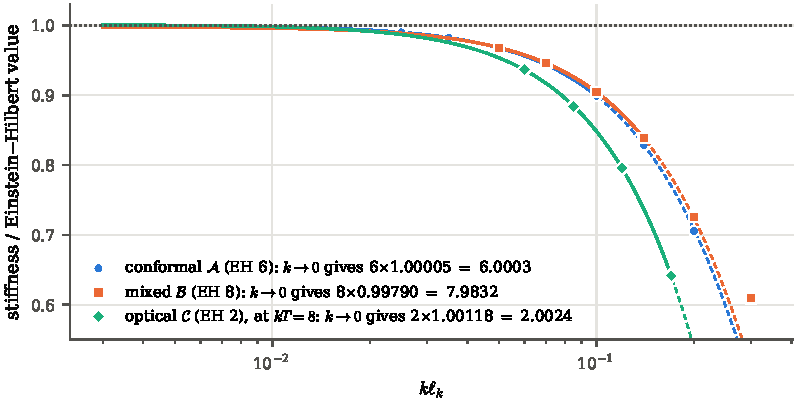
\includegraphics[width=\textwidth]{figures/fig_sectors.pdf}
  \caption{The three sectors of the static quadratic form approach the Einstein--Hilbert values as $k\to0$ (F6.8a,
F6.8b2, F6.8c2). Conformal $\cA$ and mixed $\cB$: the local part of the stiffness; optical $\cC$: $\hat K_{bb}$
at the pre-registered $n=kT=8$, which contains the age part $k^2c_0(8)$. Lines: the fits
$K_0-k^2[c_1\ln(1/k)+c_0]$ over the fitted range (solid) and continued (dashed). The intercepts give $6.0003$,
$7.983$ and $2.002$ against $6$, $8$ and $2$.}\label{fig:sectors}
\end{figure}

\paragraph{The age term of the optical sector.} Within the computed range the optical sector weakens with age
faster than linearly: at $k\ell_k=0.12$ the age part $k^2F_{bb}(n)$ grows between $n=6$, $8$, $10$, $16$ and $24$ by
increments that increase with $n$, whereas the conformal and mixed sectors become linear from $n\simeq8$
($c_T\simeq0.110$ and $0.195$). A local fit of the form $sn+qn^2$ is not stable: its coefficients depend on the
range of $n$, and they do so for the conformal sector as well below $n\simeq8$, where its linear asymptotics has
not yet set in. The data therefore do not fix the form of the optical age term; its behaviour as $kT\to\infty$,
the regime of any physical field, is open, and the predictions of the age term depend on it
(Part~\ref{part:predictions}; Fig.~\ref{fig:optical}).

\begin{figure}[t]
  \centering
  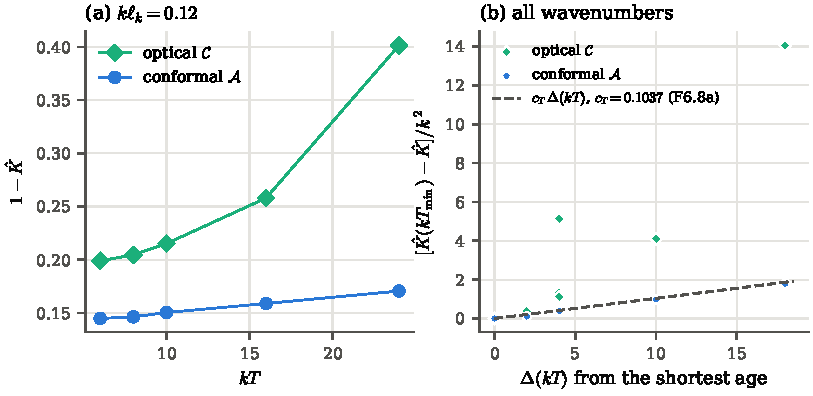
\includegraphics[width=\textwidth]{figures/fig_optical.pdf}
  \caption{The age dependence of the optical sector (F6.8c2). (a) $1-\hat K$ at $k\ell_k=0.12$ for $n=kT=6$, $8$, $10$,
$16$ and $24$, optical and conformal sectors of the same rows. (b) The decrease of $\hat K$ from the shortest
computed age, divided by $k^2$, for all wavenumbers: the conformal points follow the linear age term
$c_T\,\Delta(kT)$ of F6.8a, the optical points lie above it and grow faster than linearly.}\label{fig:optical}
\end{figure}

\subsection{What remains}

The asymptotic form of the age term in the optical sector, analytically as for the conformal one; the origin of
the differences between the sectors beyond the leading order (the age cut or the action); and the field of a
point mass by Fourier inversion of Eq.~\eqref{eq:gammaABC}. These are the next computations
(Part~\ref{part:predictions}).

% =============================================================================
\section{The static section to first post-Newtonian order}\label{sec:static}
% =============================================================================

In the rest frame of a static source the field reduces to the clock rate $\Pi$ with the metric fixed by
the throughput principle,
\begin{equation}
  \dd s^2=-\Pi^2\dd t^2+\Pi^{-2}\dd\vec x^2=-e^{2L}\dd t^2+e^{-2L}\dd\vec x^2,\qquad L=\ln\Pi .
\end{equation}
The static field equation is the BD operator of the order acting on the logarithm of the clock rate,
\begin{equation}\label{eq:static}
  B_g\ln\Pi=\kappa\rho_s
  \;\longrightarrow\;
  e^{2L}\big[(1-L)\Delta L+L|\nabla L|^2\big]=\kappa\rho_s
\end{equation}
in the continuum limit $B_g\to\Box_g-\tfrac12R$. In the weak field $\Delta L=\kappa\rho_s$, so $L=-U$ with
$\kappa\rho_s\leftrightarrow4\pi G\rho$. The choice of the logarithm is fixed by observation: for
$B_gf(\Pi)=\kappa\rho_s$ the post-Newtonian parameter is $\beta=(1-f''(1))/2$, and only $f''(1)=-1$, i.e.\ the
logarithm in the family $(\Pi^k-1)/k$, gives $\beta=1$, required by the perihelion advance. The logarithm
also turns the multiplicative composition of clock ratios into an additive potential.

This equation is the static section of the field to first post-Newtonian order ($\gamma=\beta=1$). It is not
the complete law: beyond this order the field is the full tensor field of Sec.~\ref{sec:tensor}, completed
by general relativity (Sec.~\ref{sec:jacobson}).

% =============================================================================
\section{Thermodynamic completion}\label{sec:jacobson}
% =============================================================================

Beyond the linear order the coupling to the total conserved energy--momentum, including that of the field
itself, determines the theory uniquely: it is general relativity~\cite{Deser1970,FeynmanGravitation,Lovelock1971}.
Causal Physics adopts this completion and aims to \emph{derive} it from the order, following
Jacobson~\cite{Jacobson1995}: if every local causal horizon carries an entropy proportional to its area with a
universal constant, the Clausius relation $\delta Q=T_{\rm U}\,\delta S$ for every local Rindler horizon, with the Unruh
temperature $T_{\rm U}$, implies Einstein's equations as an equation of state,
\begin{equation}
  R_{ab}-\tfrac12Rg_{ab}+\Lambda g_{ab}=8\pi G\,T_{ab},\qquad G=\frac{1}{4\hbar\eta}.
\end{equation}

What the order supplies:
\begin{itemize}
\item \emph{Entropy proportional to area.} The number of horizon molecules measures the proper area of a
  horizon (K.14, Sec.~\ref{sec:reading}).
\item \emph{Matter with energy--momentum.} Flows carry four-momentum and have a measured $T_{ab}$
  (Axiom~\ref{ax:momentum}, K.15).
\item \emph{The linear Clausius condition.} For local Rindler horizons, the Clausius relation is equivalent to
  $R_{ab}k^ak^b=8\pi G\,T_{ab}k^ak^b$ for every null direction $k$. A clock field written in a fixed frame
  violates it for moving sources; the same field written in the rest frame of each source satisfies it exactly,
  which is linearised general relativity. The condition thus requires the field to carry the four-velocity of
  its sources, which is the substrate rule of Sec.~\ref{sec:rule}.
\end{itemize}
What remains open is the Clausius relation beyond the linear order, with a dynamics of the order that responds
to matter, and the Unruh temperature~\cite{Unruh1976}, which is an input from quantum field theory. The cosmological constant
appears as an integration constant, consistently with its origin as a fluctuation of the number of events
(Sec.~\ref{sec:onto-vacuum}).


\part{Astrophysics and the Strong Field}\label{part:astro}
% =============================================================================
%  Part VII -- Astrophysics and the strong field
% =============================================================================

Astrophysics probes gravity in two directions away from the laboratory: towards strong fields
(compact objects, black holes, gravitational waves) and towards weak fields over long times and large
distances (galaxies, cosmology). This part states what Causal Physics says in each regime and where
its own content lies.

% =============================================================================
\section{The plateau is general relativity}\label{sec:astro-plateau}
% =============================================================================

On the plateau the order couples to matter as linearised general relativity
(Part~\ref{part:geometric}), and beyond the linear order the coupling to the total conserved
energy--momentum fixes the completion: general relativity. Causal Physics therefore inherits the
astrophysics of general relativity wherever geometry is a reliable description of the order:
\begin{itemize}
\item compact objects and their maximum masses, determined by general relativity and the equation of
  state of matter;
\item black holes with horizons;
\item gravitational waves with two transverse polarisations, propagating at $c$ (to $10^{-15}$ by
  GW170817~\cite{Abbott2017GW}), emitted with the quadrupole formula;
\item the perihelion advance, light deflection, Shapiro delay and frame dragging with their general
  relativistic values.
\end{itemize}
These are consistency requirements, not predictions: a measured deviation from general relativity in any
of them, at scales far above $\ell_k$, would falsify the theory (Sec.~\ref{sec:falsification}).

% =============================================================================
\section{Horizons in the causal picture}\label{sec:astro-horizons}
% =============================================================================

A black hole horizon is, in the causal picture, the limit of reconstructability
(Sec.~\ref{sec:onto-horizons}): the boundary beyond which an outside observer cannot keep an
order-preserving description of the inside. The order itself continues: causal updates go on inside,
and causal continuity is intact. \stat{interpretation}

The entropy of a horizon is a count of the order: the number of horizon molecules is proportional to its
proper area (K.14, Sec.~\ref{sec:reading}). With an entropy $s_0$ per molecule this gives the Bekenstein--Hawking law~\cite{Bekenstein1973,Hawking1975} and ties the discreteness length to Newton's
constant, $\ell\simeq1.075\sqrt{s_0}\,\ell_P$ (Sec.~\ref{sec:bridge}). \stat{tested: K.14; bridge
conditional}

What happens to the order near and inside a horizon, where the load is extreme and the geometric
reading fails, is not described by the present work. Discrete corrections to horizon physics are
expected at the scales $\ell$ and $\ell_k$. \stat{open}

% =============================================================================
\section{Discreteness and non-locality in astrophysical fields}\label{sec:astro-nonlocal}
% =============================================================================

The discrete order leaves two kinds of imprint on long-lived gravitational fields.

\paragraph{Short scales.} The static response of the order deviates from the Einstein--Hilbert form at
wavelengths approaching $\ell_k$: its spin-0 part weakens as
$1-K_{\rm loc}\simeq(k\ell_k)^2[4.0\ln(1/k\ell_k)+0.9]$ and changes sign at a wavelength of
$12.7\,\ell_k$ (Sec.~\ref{sec:bdaction}). For any $\ell_k$ far below astrophysical scales this is
invisible in astrophysics; it matters for laboratory tests of gravity at short distances
(Part~\ref{part:predictions}).

\paragraph{Long times.} The non-local age term weakens the static response of a field that has existed for
a time $T$ by the relative amount $0.1\,k^3\ell_k^2T$ (in units $c=1$). Astrophysical fields are old, and
the effect grows with their age. For the field of the Earth ($L\simeq6400$\,km, $T\simeq4.5$\,Gyr) a
relative deviation below $10^{-2}$ requires $\ell_k\lesssim1$\,mm; for the Sun at $1$\,AU and a Planckian
$\ell_k$ the effect is of order $10^{-79}$. What $T$ is in a real situation (the age of the field, the
age of the source, or the cosmological past of the region) is an open question of the theory; until it
is settled the age term constrains $\ell_k$ only conditionally. The strongest conditional bounds come not from
astrophysics but from short-range tests of gravity in the laboratory (Sec.~\ref{sec:window}). \stat{derived; interpretation of $T$ open}

\paragraph{Gravitational waves.} The same non-locality modifies the propagation of waves with wavelengths
near $\ell_k$. For astrophysical waves ($\lambda\gtrsim10^3$\,km) and any sub-millimetre $\ell_k$ the effect
is negligible. Its form for propagating waves has not been computed. \stat{open}

% =============================================================================
\section{Galaxies and cosmology}\label{sec:astro-cosmo}
% =============================================================================

\paragraph{Galaxies.} Causal Physics in its present form makes no claim about a modified regime of low
accelerations. Whether the discreteness or the non-locality of the order produces one, and at what
scale, is open. The age term weakens the response of long-lived fields at short wavelengths; it does not
strengthen gravity at large distances. In causal set theory the non-locality of the d'Alembertian has been
proposed as an origin of dark matter through off-shell modes~\cite{SaravaniAslanbeigi2015}; whether the
order of Causal Physics, or its flows, have such modes has not been studied. \stat{open}

\paragraph{The cosmological constant.} The number of events in a region fluctuates by about its square
root. Such fluctuations act on the large-scale geometry like a cosmological constant whose magnitude is
set by the four-volume of the observable universe, and for the present universe it is of the order of
the observed value~\cite{Ahmed2004}; in the thermodynamic completion it is an integration constant
(Sec.~\ref{sec:jacobson}). \stat{open}

\paragraph{Expansion.} The growth of the order on the largest scale is the natural candidate for the
expansion of the universe. A growth dynamics that produces it has not been formulated.
\stat{open}


\part{Predictions and Falsification}\label{part:predictions}
% =============================================================================
%  Part VIII -- Predictions and falsification
% =============================================================================

This part sets out what Causal Physics predicts, how each prediction is to be tested, and what would
falsify the theory. It is the programme for the next round of tests: every entry below is formulated so
that a test with a criterion fixed in advance can be written for it.

% =============================================================================
\section{What counts as a prediction}\label{sec:what-prediction}
% =============================================================================

A result is a \emph{prediction} only if it is fixed before the comparison and nothing in it was
calibrated on the data it is compared with. The results of the theory fall into three classes:
\begin{enumerate}
\item \textbf{Consistency with general relativity.} In the regime where geometry describes the order, the
  theory reproduces general relativity at the linear order and adopts it beyond. Agreement with the
  classical tests is required, not predicted.
\item \textbf{Predictions of the discreteness.} Deviations from general relativity whose \emph{shape} is
  fixed by the Benincasa--Dowker kernel and whose \emph{scale} is the single free parameter $\ell_k$.
  These are the predictions of the theory. Data either bound $\ell_k$ or detect the deviation.
\item \textbf{Structural statements.} Properties of the substrate that hold independently of $\ell_k$:
  Lorentz invariance, sharp images of distant sources, the area law of horizons.
\end{enumerate}

% =============================================================================
\section{Consistency with general relativity}\label{sec:consistency}
% =============================================================================

\begin{center}
\begin{tabularx}{\linewidth}{>{\raggedright\arraybackslash}p{3.6cm}>{\raggedright\arraybackslash}X>{\raggedright\arraybackslash}p{4.6cm}}
\toprule
quantity & origin in Causal Physics & status\\
\midrule
$\gamma=1$ & throughput principle; tensor coupling in 3+1; action of the order & derived; F7.1c raw $1.000\pm0.045$; $\cA$, $\cB$, $\cC$ emerge, $\gamma(0)=0.997$--$1.000$ (F6.8a, F6.8b2, F6.8c2)\\
$\beta=1$ & general-relativistic completion; logarithmic static section & follows from the completion; the logarithm is chosen to match it\\
frame dragging & response in the rest frame of each flow & derived; F7.4a\\
pressure gravitates as $\rho+3p$ & coupling to $T_{ab}$ & derived; F7.4a\\
quadrupole radiation, two polarisations & tensor field, GR completion & derived\\
equivalence principle & motion along the longest histories & derived; free fall along longest chains F5.1d (2+1)\\
Lorentz invariance & sprinkled substrate & structural\\
\bottomrule
\end{tabularx}
\end{center}

% =============================================================================
\section{The window of the non-locality scale}\label{sec:window}
% =============================================================================

Every prediction of the discreteness is a function of $\ell_k$, and $\ell_k$ is not free in the whole range
from the Planck length to laboratory scales.

\paragraph{Existing bounds.} The non-locality of causal set d'Alembertians has been confronted with data
for fields that propagate with the non-local operator. Comparing non-local relativistic effective field
theories with collider data at $8$\,TeV gives $\ell_k\lesssim10^{-19}$\,m, and the ground state of an
opto-mechanical oscillator gives an independent $\ell_k<2\times10^{-15}$\,m~\cite{Belenchia2016opto}.
In Causal Physics matter is a flow that carries its four-velocity, not a field propagated by $B_\epsilon$,
so whether these bounds apply to the scale of the gravitational sector depends on the matter sector,
which is open. If the same $\ell_k$ governs both, $\ell_k\lesssim10^{-19}$\,m. \stat{open}

\paragraph{Consequence for the local corrections.} For $\ell_k\lesssim10^{-19}$\,m the local correction of
Sec.~\ref{sec:bdaction}, of relative size $(k\ell_k)^2\ln(1/k\ell_k)$, is below $10^{-28}$ at the shortest
distance at which gravity is measured, $52\,\mu$m~\cite{Lee2020}: unobservable.

\paragraph{Consequence for the age term.} The age term is not suppressed in the same way. Its relative size
$\delta\simeq c_T\,k^3\ell_k^2\,T$ grows with the age $T$, and with $k=1/L$ it becomes of order one at the length
\begin{equation}\label{eq:Lstar}
  L_*=\big(c_T\,\ell_k^2\,T\big)^{1/3},\qquad c_T=0.1035 .
\end{equation}
Requiring $\delta<10^{-2}$ at $L$ gives $\ell_k\lesssim\sqrt{\delta L^3/(c_T T)}$. The outcome depends on what
$T$ is:
\begin{center}
\small
\begin{tabular}{lcccc}
\toprule
reading of $T$ & $T$ (m) & bound on $\ell_k$ & $L_*$ & $L_*$\\
 & & from $L=52\,\mu$m & ($\ell_k=\ell_P$) & ($\ell_k=10^{-19}$\,m)\\
\midrule
age of the universe & $1.3\times10^{26}$ & $1\times10^{-20}$\,m & $1.5\times10^{-15}$\,m & $51\,\mu$m\\
age of Earth's field & $4.3\times10^{25}$ & $2\times10^{-20}$\,m & $1.0\times10^{-15}$\,m & $35\,\mu$m\\
one year & $9.5\times10^{15}$ & $1\times10^{-15}$\,m & $6\times10^{-19}$\,m & $21$\,nm\\
one day & $2.6\times10^{13}$ & $2\times10^{-14}$\,m & $9\times10^{-20}$\,m & $3$\,nm\\
\bottomrule
\end{tabular}
\end{center}
If $T$ is cosmological, short-range tests of gravity probe $\ell_k$ at the level of collider bounds, and the
theory says where the deviation sits: at $L_*$, which for $\ell_k=10^{-19}$\,m lies at tens of micrometres,
the range of current torsion balances. If $T$ is the age of a laboratory source, the age term is out of reach.
What $T$ is (Sec.~\ref{sec:discreteness-predictions}, P2) therefore decides whether the theory is testable
at short distances now (Fig.~\ref{fig:window}). \stat{derived; conditional on the reading of $T$}

\begin{figure}[t]
  \centering
  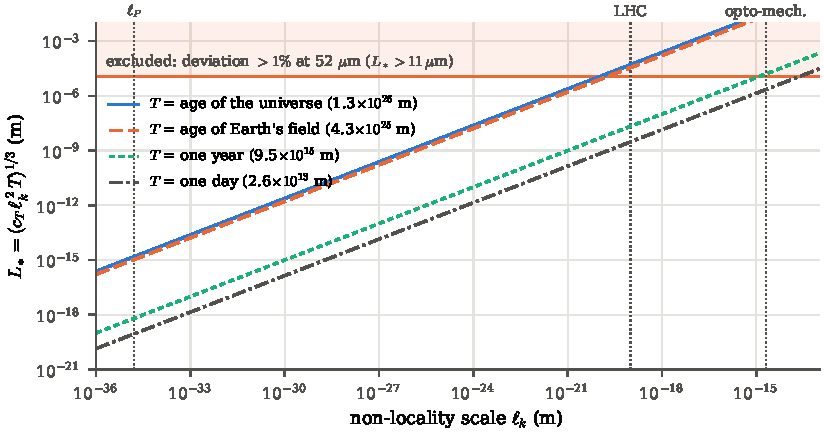
\includegraphics[width=\textwidth]{figures/fig_window.pdf}
  \caption{The window of the non-locality scale, Eq.~\eqref{eq:Lstar}: the length $L_*$ at which the age term becomes of
order one, against $\ell_k$, for the four readings of $T$. Shaded: excluded by short-range tests of gravity if
the deviation must stay below $1\%$ at $52\,\mu$m ($L_*>11\,\mu$m). Dotted: the Planck length and the bounds on
$\ell_k$ from colliders and opto-mechanics (if the same $\ell_k$ governs matter). The curves use the linear age
term of the conformal sector, $c_T=0.1035$ (caveat (i)).}\label{fig:window}
\end{figure}

\paragraph{Caveats.} (i) The estimate uses the linear age term of the conformal sector. The optical sector
weakens faster than linearly within the computed range ($kT\le24$, Sec.~\ref{sec:optical}); if this persists
as $kT\to\infty$, the breakdown moves to larger scales and the bounds become stronger. The asymptotic form decides the far-field law. (ii) In the mixed sector the age term is $1.78$ times stronger than in the
conformal one (Sec.~\ref{sec:mixed}); a covariant action cannot do this, and the difference may come from
the age cut rather than from the action. (iii) At $L_*$ the expansion in the age term breaks down, and what
happens there (Sec.~\ref{sec:discreteness-predictions}, P3) is open. The numbers above are orders of
magnitude, not a verdict.

% =============================================================================
\section{Predictions of the discreteness}\label{sec:discreteness-predictions}
% =============================================================================

\subsection{P1: the static field of a point mass near \texorpdfstring{$\ell_k$}{l\_k}}

The static field of a point mass is fixed by the three coefficients $\cA$, $\cB$, $\cC$ of the static
quadratic form of the action of the order (Sec.~\ref{sec:mixed}), without assuming covariance:
\begin{equation}
  \gamma(k,T)=\frac{\cB}{2\cC}-1,\qquad
  \frac{\Phi(k)}{\Phi_{\rm GR}(k)}=\frac{-2}{\cA-\cB^2/(4\cC)} .
\end{equation}
\begin{itemize}
\item \emph{Known:} the conformal coefficient $\cA=6\hat K(k,T)$, with
  $K_{\rm loc}=1-(k\ell_k)^2[4.0\ln(1/k\ell_k)+0.9]+\dots$ for $k\ell_k\le0.1$ and the values of
  Sec.~\ref{sec:bdaction} beyond; the mixed coefficient $\cB=8\hat K_{ab}(k,T)$, equal to $8\hat K$ at leading
  order and larger by $\simeq8\times0.46\,(k\ell_k)^2$ beyond it (Sec.~\ref{sec:mixed}); the optical coefficient
  $\cC=2\hat K_{bb}(k,T)$, with $\cC(k\to0)=2.002$ and an age dependence that grows faster than linearly in the
  computed range (Sec.~\ref{sec:optical}).
\item \emph{To compute:} the asymptotic form of the optical age term, $kT\to\infty$.
\item \emph{Prediction:} the potential $\Phi(r)$ and $\gamma(r)$ of a point mass as functions of
  $r/\ell_k$, by Fourier inversion. The shape is fixed; only $\ell_k$ is free.
\item \emph{Test:} laboratory searches for deviations from the inverse-square law at sub-millimetre
  distances (torsion balances~\cite{Lee2020}), and light deflection and Shapiro delay at the largest $k$
  accessible. If $\ell_k$ obeys the existing bounds (Sec.~\ref{sec:window}), the local part of P1 is out of
  reach and its observable content is the age term.
\item \emph{Falsification:} if the predicted shape is excluded by the data for every $\ell_k$ above the
  discreteness length $\ell$, the theory fails.
\end{itemize}

\subsection{P2: the age term}

A static field that has existed for a time $T$ responds more weakly at wavenumber $k$ by the relative
amount
\begin{equation}
  \frac{\delta\hat K}{\hat K}\simeq-0.10\,k^3\ell_k^2\,T\qquad(c=1).
\end{equation}
\begin{itemize}
\item \emph{Status:} derived analytically and confirmed by the full computation to $2\%$, in the static
  conformal sector (F6.8a). In the mixed sector it is $1.78$ times larger, $c_{T,ab}\simeq0.195$
  (F6.8b2): the age term does not enter the sectors in covariant proportion. In the optical sector it grows
  faster than linearly within the computed range, $kT\le24$ (F6.8c2), with a form the data do not fix; it
  therefore shifts $\gamma$ as well as the strength of the field. Its form as $kT\to\infty$ is open.
\item \emph{Open:} what $T$ is physically (age of the field, of the source, or the cosmological past),
  and the form of the term in the full static propagator.
\item \emph{Consequence:} requiring a relative deviation below $\delta$ at scale $L$ gives
  \begin{equation}
    \ell_k\lesssim\sqrt{10\,\delta\,L^3/T},
  \end{equation}
  e.g.\ $\ell_k\lesssim1$\,mm from the field of the Earth at the scale of its radius ($\delta=10^{-2}$). At the
  shortest tested distance, $52\,\mu$m, the bound ranges from $10^{-20}$\,m (cosmological $T$) to
  $2\times10^{-14}$\,m ($T$ of one day); Sec.~\ref{sec:window}.
\item \emph{Caveat:} the age term enters the conformal and mixed sectors in a non-covariant proportion; it may
  come from the way the past is cut at age $T$ rather than from the action. A test of this is planned
  (F6.8d).
\item \emph{Test:} comparison of the strength of gravity of fields of different ages at the same scale,
  e.g.\ freshly assembled laboratory masses against the field of the Earth.
\end{itemize}

\subsection{P3: the static pole of the spin-0 channel}

The spin-0 propagator has a static pole where $\hat K=0$. Without the age term it lies at a wavelength
of $12.7\,\ell_k$; with it, at the length scale $L_*=(0.1\,\ell_k^2T)^{1/3}$ of Eq.~\eqref{eq:Lstar}, which for
$T$ equal to the age of the universe is $\sim10^{-15}$\,m for a Planckian $\ell_k$ and $\sim50\,\mu$m for
$\ell_k=10^{-19}$\,m. Whether the pole signals a standing wave, an
instability of the static sector, or the limit of validity of the expansion is open. \stat{open}

\subsection{P4: the cosmological constant}

The fluctuation of the number of events gives a cosmological constant of the observed order of magnitude
that varies over cosmic time~\cite{Ahmed2004}. This is a known prediction of causal set theory that
Causal Physics shares. \stat{open}

% =============================================================================
\section{Structural predictions}\label{sec:structural}
% =============================================================================

\begin{itemize}
\item \textbf{Exact Lorentz invariance of the substrate.} No preferred frame at any scale. A detected
  violation of Lorentz invariance would contradict Axiom~\ref{ax:substrate}. A Lorentz-invariant discrete
  substrate can still make particles diffuse slowly in momentum (``swerves''~\cite{DowkerHensonSorkin2004});
  for flows that carry their four-velocity this has not been computed. \stat{open}
\item \textbf{No blurring of distant point sources by the discreteness.} Influence on the light cone
  passes no intermediate events, so the images of distant quasars and gamma-ray bursts are not blurred
  by the substrate. Observed sharp images agree with this; a detected discreteness-induced blurring would
  contradict it.
\item \textbf{Horizon entropy proportional to proper area,} with the discreteness length tied to $G$
  through $s_0$ (Sec.~\ref{sec:bridge}).
\end{itemize}

% =============================================================================
\section{Falsification}\label{sec:falsification}
% =============================================================================

The theory is falsified, in the sense that its present form must be abandoned, if any of the following
holds:
\begin{enumerate}
\item a deviation from general relativity is measured in the classical tests (light deflection,
  Shapiro delay, perihelion advance, frame dragging, binary pulsars, gravitational-wave polarisations)
  at scales far above any admissible $\ell_k$;
\item the $\nu^2$ sector of the discrete action gives a long-wavelength coefficient $\cC$ different from
  $2$: then $\gamma=\cB/(2\cC)-1\neq1$ at large scales, $\gamma=1$ does not follow from the action of the order,
  and the substrate rule is an independent postulate (checked: $\cB\to7.983$, $\cC\to2.002$, passed);
\item the static field of a point mass predicted from the three coefficients $\cA$, $\cB$, $\cC$ is excluded by
  short-range gravity data for every $\ell_k\ge\ell$;
\item a violation of Lorentz invariance of the substrate is detected;
\item the images of distant point sources are found blurred in a way attributable to the discreteness
  of spacetime.
\end{enumerate}

% =============================================================================
\section{The next tests}\label{sec:next-tests}
% =============================================================================

\begin{center}
\begin{tabularx}{\linewidth}{>{\raggedright\arraybackslash}p{1.3cm}>{\raggedright\arraybackslash}X>{\raggedright\arraybackslash}p{3.0cm}}
\toprule
test & question & needs\\
\midrule
F6.8e & the asymptotic age term of the optical sector, $kT\to\infty$ (analytic, as for $c_T$) & F6.8c2\\
F6.8d & the differences between the sectors beyond leading order: from the age cut or from the action? & F6.8b2\\
F8.1 & $\Phi(r)$, $\gamma(r)$ of a point mass in units of $\ell_k$; comparison with short-range data & F6.8e\\
F8.8 & the physical meaning of the age $T$; fields of different ages & theory of $T$\\
F6.9 & the age term in the full static propagator & F6.8c\\
\bottomrule
\end{tabularx}
\end{center}
Each of these will be registered with its criterion before it is run, and its outcome reported whatever it
is.


\part{Discussion and Conclusion}\label{part:discussion}
% =============================================================================
%  Part IX -- Discussion and conclusion
% =============================================================================

\section{What has been shown}\label{sec:shown}

Starting from events and their order, Causal Physics reaches the following, each step tested or derived:
\begin{enumerate}
\item The substrate is a Lorentz-invariant causal set, and its geometry can be read blindly from order and
  number.
\item Matter is a flow that carries its four-velocity; localisation requires this memory, and the memory is
  inertia. The flows have a conserved energy--momentum tensor.
\item The order responds to matter, and the way it responds fixes $\gamma$: a fixed order gives
  $\gamma=-1$, narrowing cones give $\gamma=1/d_s$, conservation of throughput gives $\gamma=2/(d_s-1)$,
  which is $1$ in three spatial dimensions.
\item In three spatial dimensions the throughput principle is the coupling of linearised general relativity
  to $T_{ab}$, and a substrate rule realising it makes pressure and motion gravitate and drags the cones.
\item That rule is not an independent postulate: with the proper time of a flow counted by the order, it is
  the linear response of an order whose action has the Einstein--Hilbert stiffness.
\item The discrete Benincasa--Dowker action has that stiffness: $6.0003$ against $6$ in the static
  conformal sector, $7.983$ against $8$ in the mixed sector and $2.002$ against $2$ in the optical
  sector, computed with nothing from general relativity put in; $\gamma=1$ follows from it. The discreteness
  adds a non-analytic correction and non-local terms that grow with the age of the field, and beyond the
  leading order the sectors differ.
\end{enumerate}

\section{Limitations}\label{sec:limitations}

\begin{itemize}
\item \textbf{Expected values, not dynamics.} The action of the order is evaluated as an expectation over
  sprinklings of a given geometry. That a dynamics of the order selects such causal sets, the manifold-like
  phase, is assumed, as in causal set theory generally.
\item \textbf{Finite ages.} The coefficients are computed for ages up to a few hundred $\ell_k$; the age term of
  the optical sector grows faster than linearly there, and its asymptotic form is not known. Beyond the
  leading order the sectors are not in covariant proportion; whether this comes from the age cut or from the
  action is open.
\item \textbf{The substrate rule as an input in the tests.} The tests of the coupling (F7.1c, F7.4a) build
  the order according to the rule. They show what the rule implies, not that nature uses it; the
  derivation from the action supplies the reason.
\item \textbf{Matter as a self-bound object.} Flows are localised by their memory of direction, but a
  particle that holds itself together without an external source has not been obtained.
\item \textbf{The quantum.} The theory is classical. Superposition and measurement have an
  interpretation, not a dynamics.
\item \textbf{The age term.} Its coefficient is established; its physical reading, what $T$ is, is not, and
  it may depend on how the past is cut. The reading decides whether short-range gravity tests probe $\ell_k$ now
  (Sec.~\ref{sec:window}).
\item \textbf{The scale $\ell_k$.} Existing bounds on non-local fields give $\ell_k\lesssim10^{-19}$\,m. Whether
  they apply to the gravitational sector depends on the matter sector, which is open.
\item \textbf{Finite numerics.} Laboratory results come from finite regions and finite numbers of
  sprinklings, with the limits stated in each test.
\end{itemize}

\section{Outlook}\label{sec:outlook}

The road from here to predictions is short and concrete: the asymptotic age term of the optical sector,
then the static field of a point mass from the three coefficients, compared with short-range gravity data,
and the physical meaning of the age $T$. In parallel, the thermodynamic route is to turn the completion by general relativity from
an adopted principle into a derived one, and the matter sector is to find the self-bound flow.

\section{Conclusion}\label{sec:conclusion}

Gravity in Causal Physics is the response of a causal order to the matter that flows through it. The
order slows its clocks, narrows its cones and adds events so that its throughput is kept, and in three
spatial dimensions this is exactly the coupling of general relativity. The reason is the action of the
order itself: counting the intervals of a causal set gives the Einstein--Hilbert stiffness, and the
counting also says where it stops being exact. That is where the predictions of the theory are.


\appendix
\part*{Appendices}
\addcontentsline{toc}{part}{Appendices}
\section{The Causality Lab}\label{app:lab}

\subsection{Purpose and architecture}

The Causality Lab~\cite{CausalityLab} is an open Python code base written to test Causal Physics step by
step. It has three layers:
\begin{itemize}
\item a \emph{core}: sprinkling of causal sets in 1+1 to 3+1 dimensions, causal relations and links,
  interval counts, the discrete and expected Benincasa--Dowker operator and action (flat and curved),
  transport of flows with capacity and carried four-velocity, and blind instruments that read geometry
  from the order;
\item \emph{tests}, one file per test, each with a header that states the question, method, prediction,
  null model, criterion, level of conclusion, the instruments it depends on and an estimate of its cost;
\item a \emph{runner} that executes a test (\texttt{python run.py <ID>}), records the full parameters, the
  seed, the version and the output, and refuses to change the criteria of a full run.
\end{itemize}
Deterministic computations (expected values by quadrature) carry their own convergence checks; stochastic
ones (sprinklings) are replicated with independent seeds before a verdict is final.

\subsection{Rules}

The methodological principles M1--M7 (Sec.~\ref{sec:method-ax}) are enforced by the runner and the test
headers; a revision of a test states its reason in its header. Calibrations (phase K) establish
instruments and carry no physical conclusion.

\subsection{Tests cited in this paper}

\begin{center}
\small
\begin{tabularx}{\linewidth}{>{\raggedright\arraybackslash}p{1.9cm}>{\raggedright\arraybackslash}X>{\raggedright\arraybackslash}p{3.0cm}}
\toprule
test & question and result & verdict\\
\midrule
K.1 & geometry readable from the order in 3+1 from $N\approx3\times10^4$ & calibration\\
K.2 & causal front measures the Shapiro delay ($0.98$ of GR) and deflection ($0.84$--$0.87$) & calibration\\
K.3 & clock rate readable from the density of chains & calibration, replicated\\
K.11, K.11c & curved BD operator tends to $\Box_g-\tfrac12R$ (conformal geometry, near and far field) & calibration\\
K.13a & BD operator in a geometry with bent light converges, density and cone parts separately & calibration\\
K.14 & horizon molecules measure the proper area (exponent $1.96\pm0.06$ in 3+1) & calibration\\
K.15 & energy--momentum tensor of flows; four-momentum conserved exactly by $F=|P|$ & calibration, replicated\\
K.16b, K.16c & blind instrument reads $\gamma=-1,0,1$ (2+1) and $-1,\tfrac13,1$ (3+1) & calibration\\
F0.3 & degree of an event grows with $N$: no bound $K_0$ & mechanism\\
F1.1 & Gauss's law for a steady source, $J/S=1.003$--$1.004$ & mechanism\\
F1.3 & far field of a source: Green function with Gauss strength & mechanism\\
F1.4 & superposition fails at second order as predicted & mechanism, passed\\
F1.8 & capacity limits the flow, not the number of relations & mechanism (seed-sensitive)\\
F2.2, F2.4, F2.5 & maximal chains follow the geodesics of $\Pi^2\eta$ (2+1, 3+1) & mechanism, passed\\
F3.6 & a flow with carried direction is localised and moves with its source & mechanism, passed, replicated\\
F4.1 & flows that meet head-on stick: merged fraction $0.82$ (2+1), $0.77$ (3+1), merged flow at rest, no bounce & mechanism, passed\\
F5.1 & free fall with a direction carried in flat coordinates, or keeping to the longest chains from the origin: no fall & mechanism, instrument failed; failed\\
F5.1c & longest-chain history started at rest: inward, $R=0.34\pm0.05$ & mechanism, failed\\
F5.1d & longest-chain history started at the apex of a thrown ball falls, $R=1.069\pm0.051$ (2+1) & mechanism, passed\\
F5.1e & the same in 3+1 does not fall, $R=-0.13\pm0.12$; longest chains read the geometry, $R_{\max}=0.85$ & mechanism, failed\\
F6.1, F6.2 & local growth with bounded degree: no manifold, no 3D space & mechanism\\
F6.4a & 2D orders with BD action: manifold phase and transition reproduced; height of the crystalline
  phase not & calibration, failed\\
F6.8a & EH stiffness of the expected BD action, $6.0003$; correction and age term & chain, passed\\
F6.8b2 & mixed stiffness, $7.983$ against $8$; covariant at leading order, sectors differ beyond (revision of F6.8b, whose instruments failed) & chain, passed\\
F6.8c & optical sector read linearly in the age: the age dependence is not linear & chain, failed\\
F6.8c2 & optical sector read at fixed $kT$ on new wavenumbers: $\cC(0)=2.002$ against $2$ & chain, passed\\
F7.1a & cones narrowed without added events give $\gamma\approx\tfrac12$ (2+1), as derived & mechanism, failed\\
F7.1b & throughput principle in 2+1: $\gamma\approx1.85$ against $2$ & mechanism, undecided\\
F7.1c & throughput principle in 3+1: $\gamma=1.000\pm0.045$, $0.972\pm0.074$ & mechanism, undecided\\
F7.4a & tensor coupling of counter-streaming flows, $R=2.401\pm0.053$ against $2.361$ & mechanism, passed\\
\bottomrule
\end{tabularx}
\end{center}
A verdict answers the question the test asked. \verdict{failed} for F7.1a means that cones which only
narrow do not give $\gamma=1$, which was the derived expectation; \verdict{undecided} for F7.1b and F7.1c
means that the statistical comparison with the control metric was too weak for a formal verdict, while the
raw values agree with the prediction.

\subsection{Availability}

The code, the test headers and the recorded outputs of every run quoted here are available at
\url{https://github.com/pavelsikula92/Causal-Lab-}. Every number in this paper can be reproduced with \texttt{python run.py <ID>}.

\section{Relation to the first version}\label{app:changes}

The first published version of this programme~\cite{Sikula2026v1} stated it in a broad form. This
appendix relates the two: what is kept, what is reformulated, and what is no longer claimed. Every change
results from a test or a derivation in the present work.

\subsection{Kept}

\begin{itemize}
\item The primacy of causality over geometry; events without intrinsic properties; the causal order as
  the deepest structure.
\item Causal continuity: influence is conserved at every event.
\item Finite capacity, now as a bound on the flow through an event.
\item The local response variables $\Pi_v$, $I_v$ and $Z_v=I_v/\Pi_v$, and the Causal Resistance
  Functional as the action of a flow.
\item The picture of $c$ as the maximal congestion-free throughput and of $c_{\rm eff}$ falling where the
  substrate is loaded. It is now the throughput principle, which gives $\gamma=1$ in three spatial
  dimensions.
\item The separation of the causal, bridge and observational layers.
\item The ontological themes: observation and causal resolution, branching and merging, horizons as
  limits of reconstructability, superposition as coexisting continuations.
\end{itemize}

\subsection{Reformulated}

\begin{itemize}
\item \textbf{The substrate.} A graph with bounded degree $K_0$, locality by graph distance and time as a
  count of updates has a rest frame. It is replaced by a Lorentz-invariant causal set, as required by the
  theorem of Bombelli, Henson and Sorkin and supported by the tests F0.3, F1.8, F6.1 and F6.2.
\item \textbf{Dimension.} The effective dimension is no longer defined by the growth of graph balls; it is
  read from the order (fraction of related pairs, blind instruments).
\item \textbf{The dynamical principle.} The Causal Resistance Functional is the action of a flow; the
  dynamics of the order is the Benincasa--Dowker action.
\item \textbf{Gravity.} The inverse-square law from flux through spherical shells is replaced by the
  response of the order: clocks, cones and density, with the tensor coupling derived and tested.
\item \textbf{Special relativity.} The Lorentz factor is no longer derived from clocks at rest relative to
  the substrate; Lorentz invariance is a property of the substrate.
\item \textbf{Gravity changes the causal order.} Near matter the cones narrow and events are added;
  causality itself (no loops, conservation of flow) is untouched.
\end{itemize}

\subsection{No longer claimed}

\begin{itemize}
\item The cosmological anchor $a_0=cH_0/2\pi$ and the low-acceleration regime built on it, including the
  reinterpretation of dark matter. The anchor is not derived from the present formulation, and its
  mechanism relied on the bounded-degree substrate.
\item The plateau $D_{\rm eff}\approx3$ as an attractor of a bounded-degree dynamics.
\item Threshold effects in strong gravity (suppression of the redshift of white dwarfs, environment-dependent
  delays of gravitational waves), and strong-field properties of a scalar field equation. Beyond the
  linear order the theory is completed by general relativity.
\item The projection of time and length through the Hubble scale and the projection of impedance through the
  vacuum electromagnetic impedance.
\end{itemize}


\section*{Acknowledgements}
\addcontentsline{toc}{part}{Acknowledgements}
The analyses, the code of the Causality Lab and this text were developed with the assistance of an AI
system (Claude, Anthropic). All numerical results were produced by the tests of the laboratory, whose
code and outputs are public, and were checked by the author, who takes responsibility for the content.
\todo{edit or remove as the author prefers}

\section*{Funding}
\addcontentsline{toc}{part}{Funding, competing interests, data and licence}
This work received no external funding.

\section*{Competing interests}
The author declares no competing interests.

\section*{Data and code availability}
The code of the Causality Lab, the headers of all tests with their pre-registered criteria, and the
recorded outputs of every run quoted in this paper are available at
\url{https://github.com/pavelsikula92/Causal-Lab-}. The version used for this paper is archived as
\todo{release tag and Zenodo DOI of the code}.

\section*{Licence}
This work is distributed under the Creative Commons Attribution 4.0 International licence (CC BY 4.0).

\bibliographystyle{unsrtnat}
\bibliography{references}
\end{document}
